\label{sec:gbb-bkgres}
%%%%%%%%%%%%%%%%%%%%%%%%%%%%%%%%%%%%

The flavor fraction fits are performed in each bin of each observable to determine the $b\bar b $ fractions in data. For \drbb, fits are performed in $\drbb \in\{[0.2, 0.25], [0.25, 0.3], [0.3, 0.4], [0.4,0.5], [0.5,0.6], [0.6,0.7]\}$. For \zpt, fits are performed in $\zpt \in\{[0, 0.1], [0.1, 0.2], [0.2, 0.3], [0.3,0.4], [0.4,0.5]\}$. For \mpt, fits are performed in $\mpt \in\{[-3, -2.2], [-2.2, -1.9], [-1.9, -1.5], [-1.5, -1.1], [-1.1,0]\}$. For \dphi, fits are performed in $\dphi \in\{[0, \pi/5], [\pi/5, 2\pi/5], [2\pi/5, 3\pi/5], [3\pi/5, 4\pi/5], [4\pi/5, \pi]\}$. Examples of post-fit Data/MC comparisons for each variable are shown in Fig.~\ref{fig:fit-example}. Refer to \ref{sec:app-subsd0fits} for all pre-fits and post-fits data-MC comparisons. The MC predicted and fitted fraction of each flavor component are shown in Fig.~\ref{fig:gbb-fitfrac}.

Four sets of fit cross check are performed: (1) using \sdzero as discriminant (2) using \subsubsdzero (3) using $p_T$ parameterized templates and (4) with track jet kinematic re-weighting. The cross check results are summarized in Fig.~\ref{fig:dR-fitfrac-crosscheck}\ref{fig:ZpT-fitfrac-crosscheck}\ref{fig:fracmasspt-fitfrac-crosscheck}\ref{fig:dphi-fitfrac-crosscheck}. We observe closure of the fitted signal (`BB' component) event fraction in all the cross checks within fitting uncertainties. The size of each of the systematic uncertainty is summarized in Table ~\ref{tab:dRsys}\ref{tab:ZpTsys}\ref{tab:fracmassptsys}\ref{tab:dphisys}.

\begin{figure}[htbp]
  \centering
 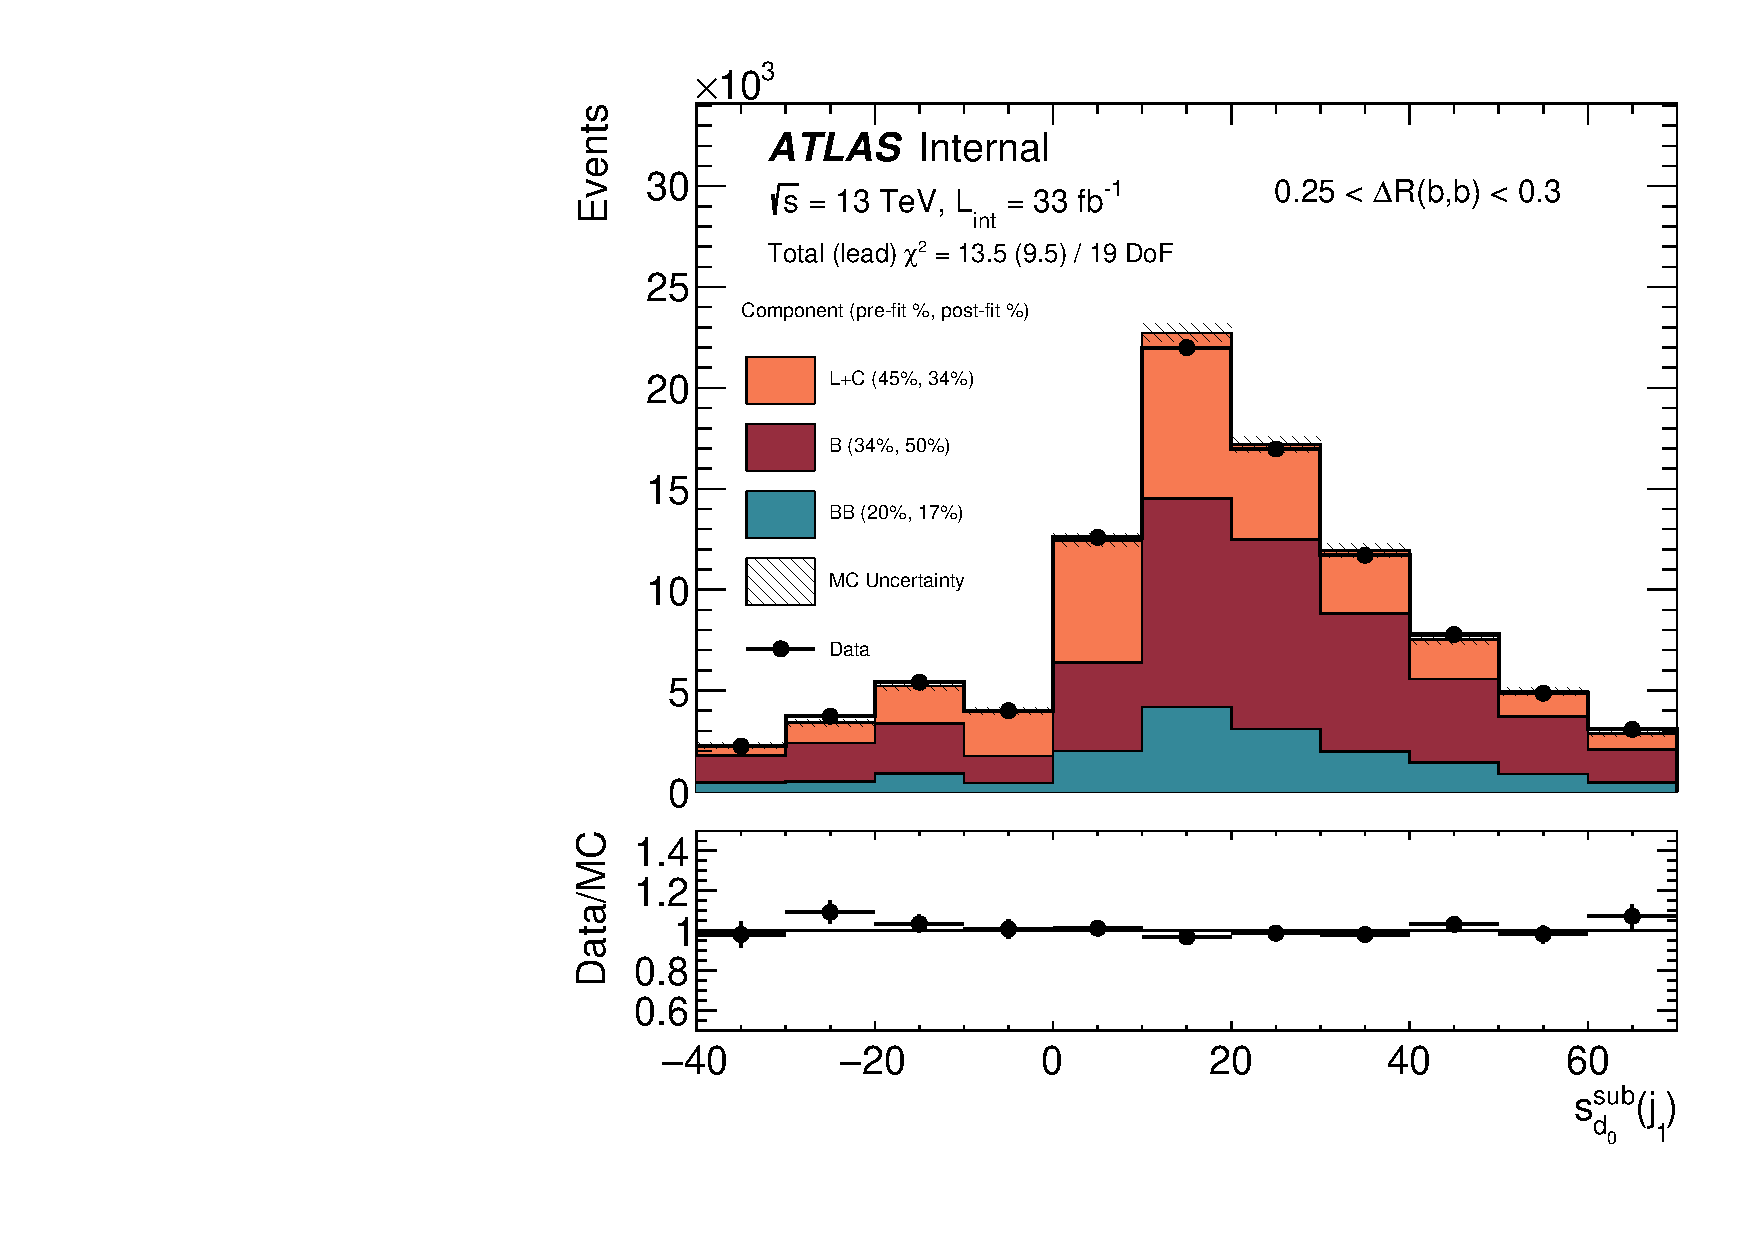
\includegraphics[width=0.45\textwidth]{figures/gbb/paperplots/Canv_Fit_dR_LpT_INF_SpT_INF_coarse_x}
 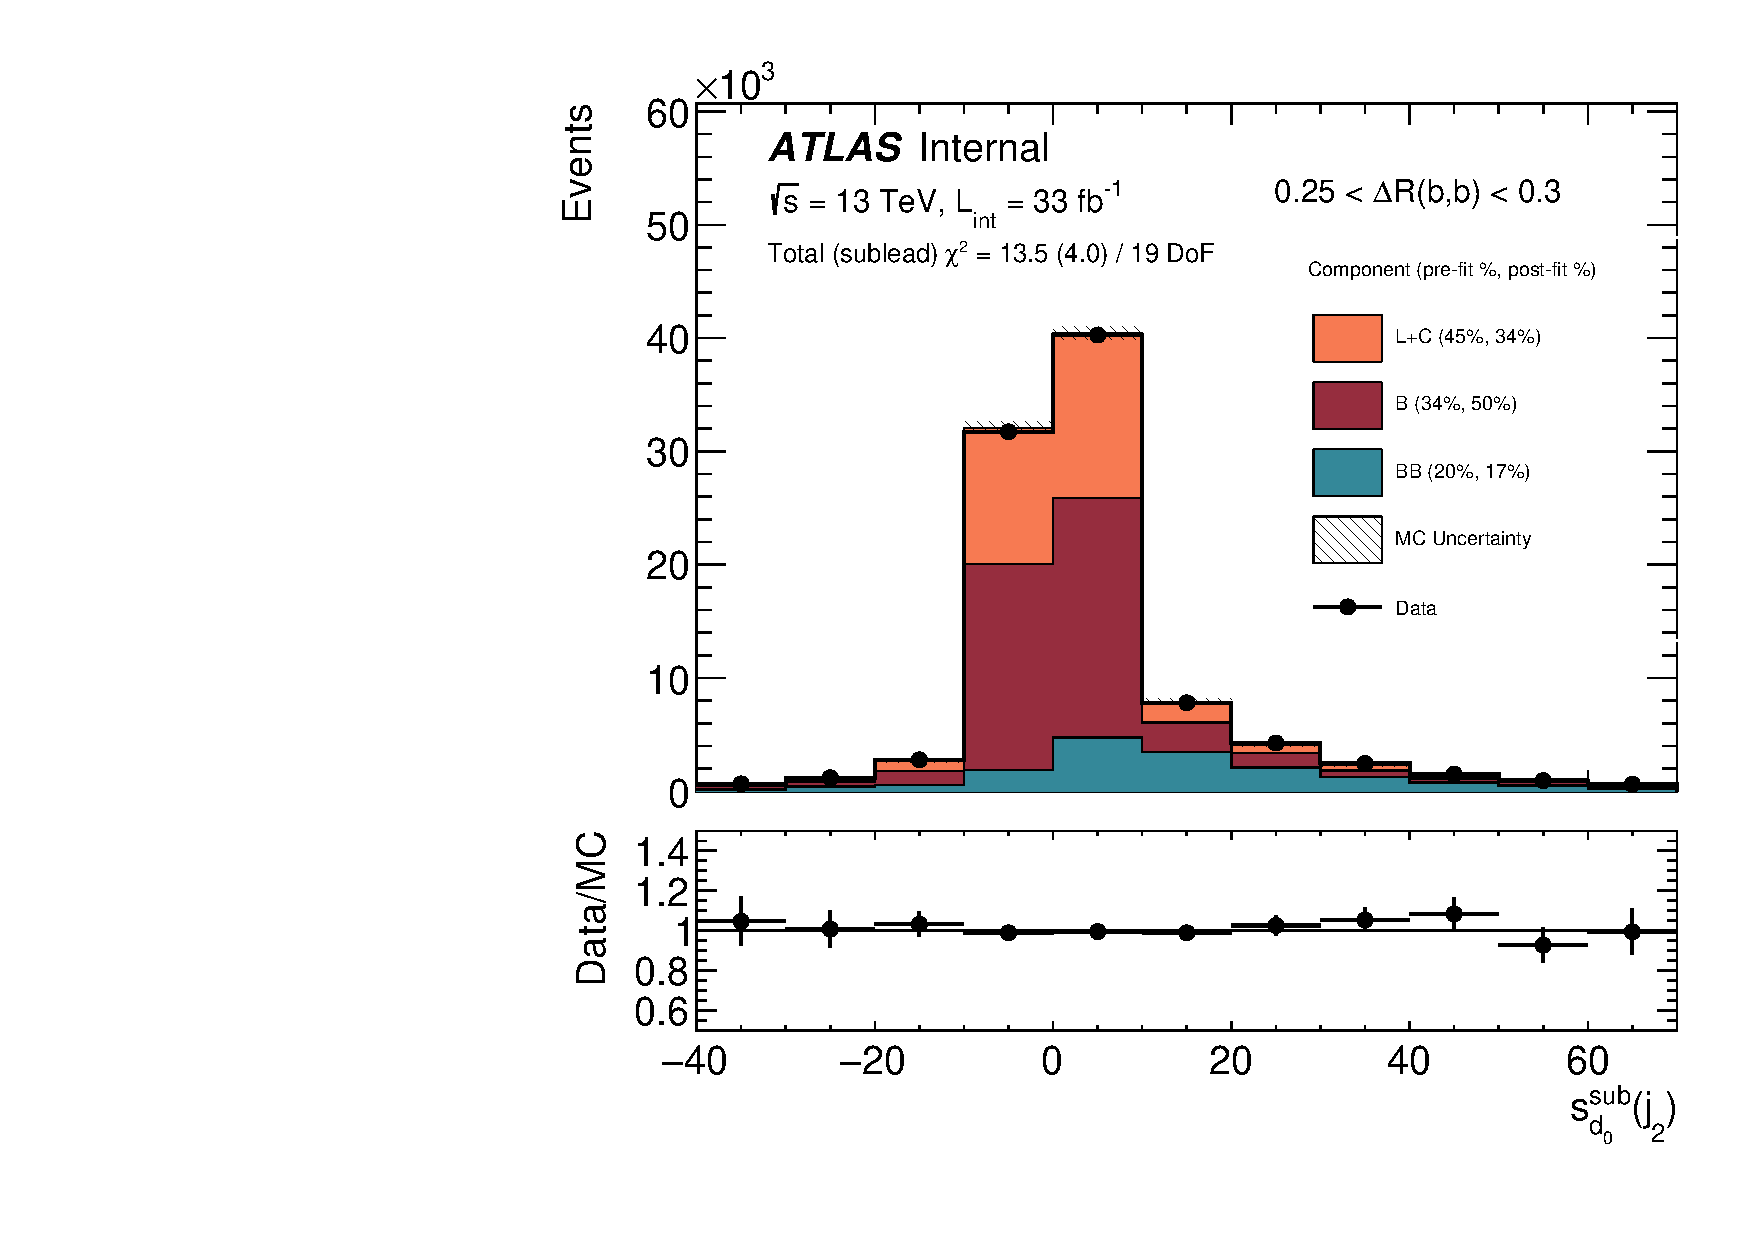
\includegraphics[width=0.45\textwidth]{figures/gbb/paperplots/Canv_Fit_b0_25_DeltaR_0_3_LpT_INF_SpT_INF_coarse_y}
 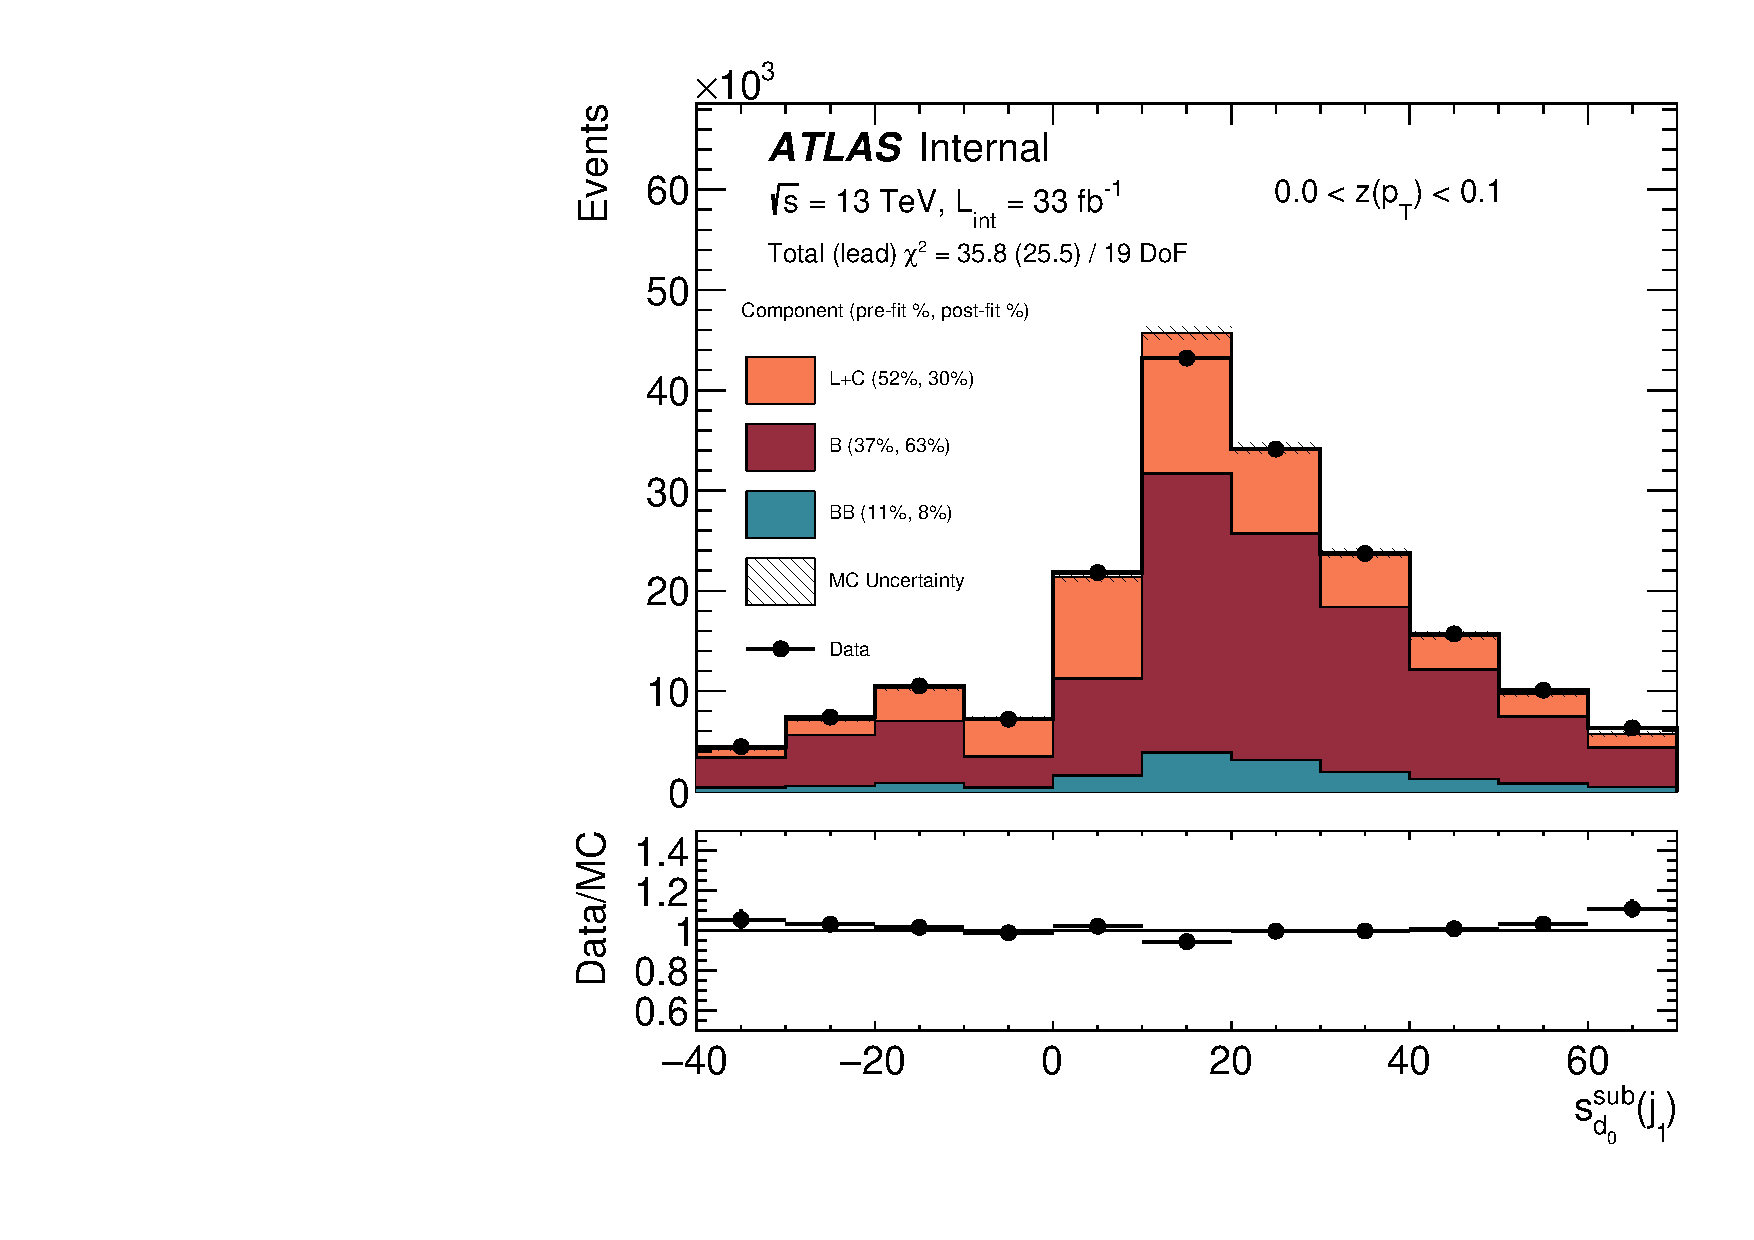
\includegraphics[width=0.45\textwidth]{figures/gbb/paperplots/Canv_Fit_zpt_LpT_INF_SpT_INF_coarse_x}  
 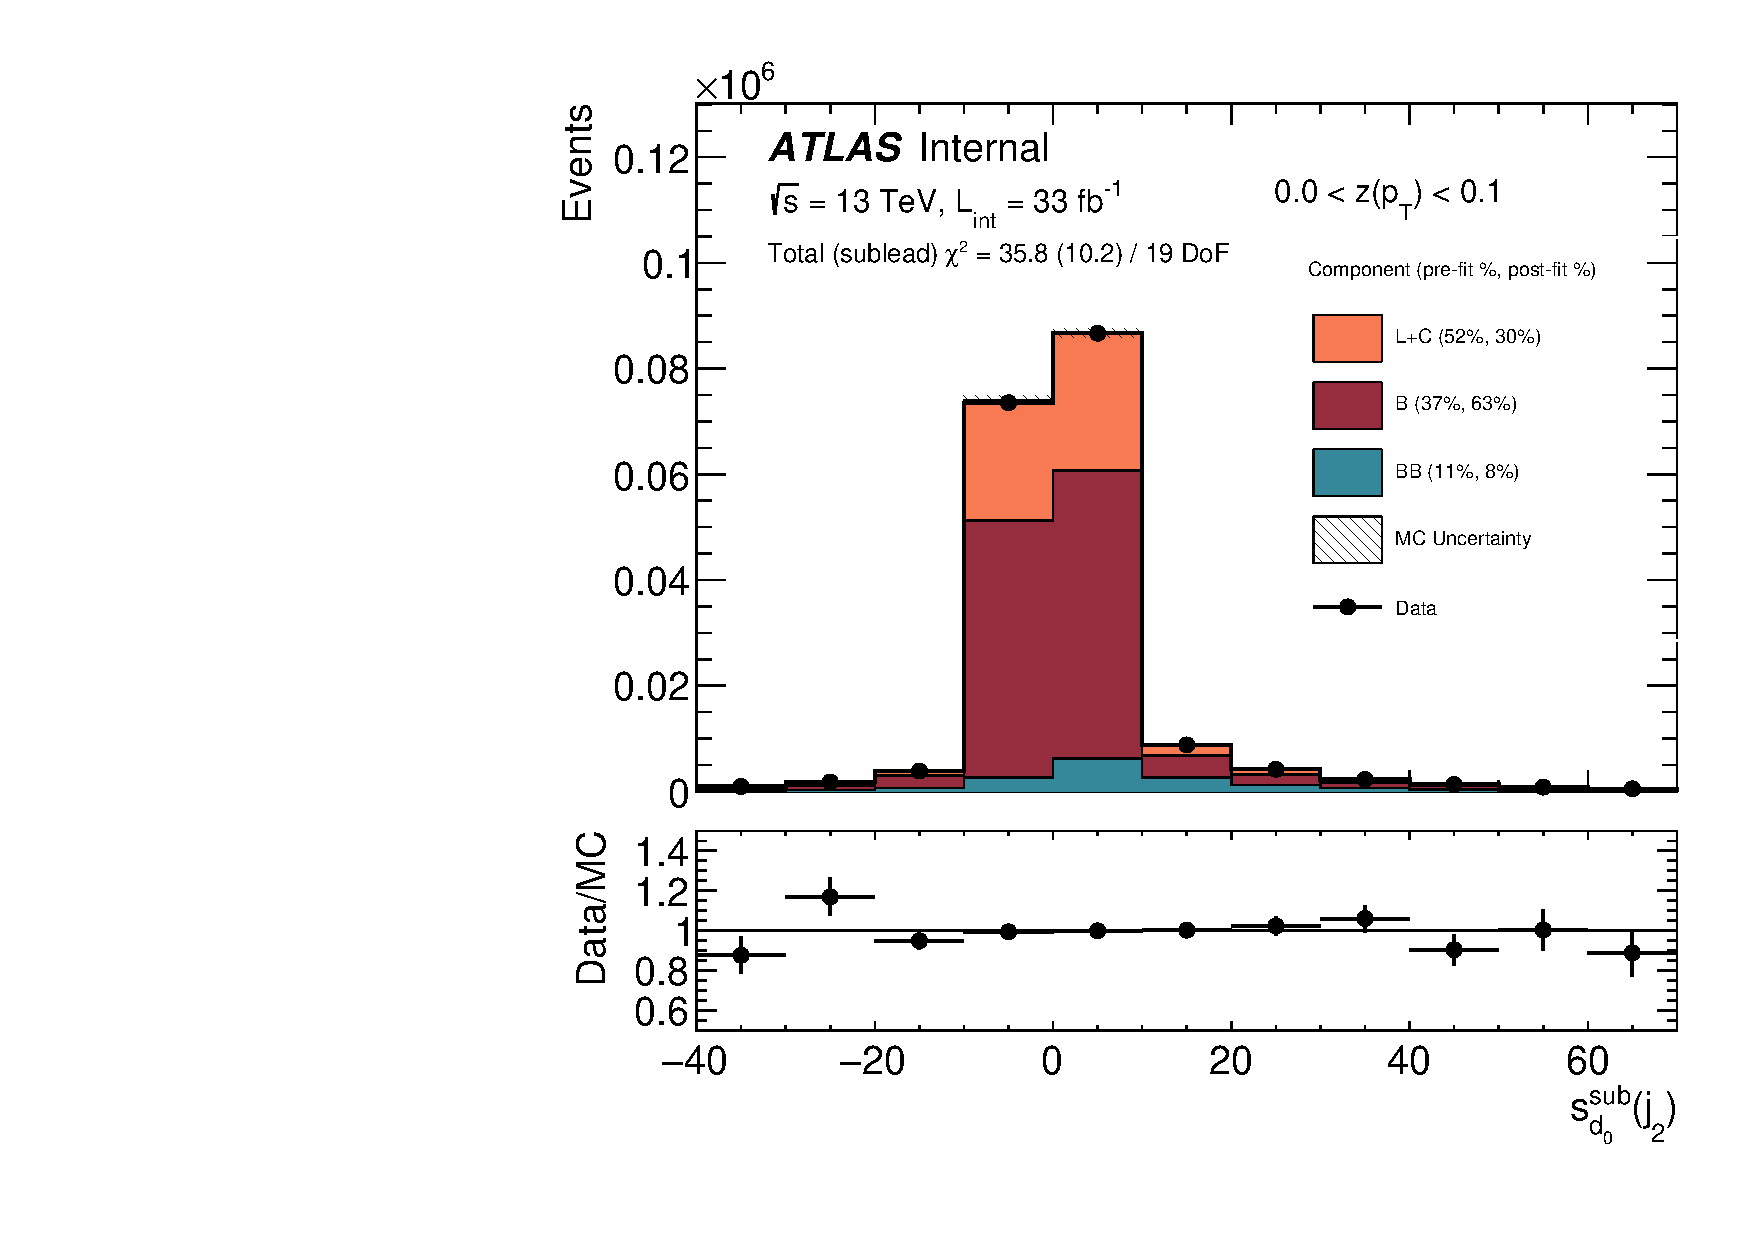
\includegraphics[width=0.45\textwidth]{figures/gbb/paperplots/Canv_Fit_b0_25_zpt_0_3_LpT_INF_SpT_INF_coarse_y}
 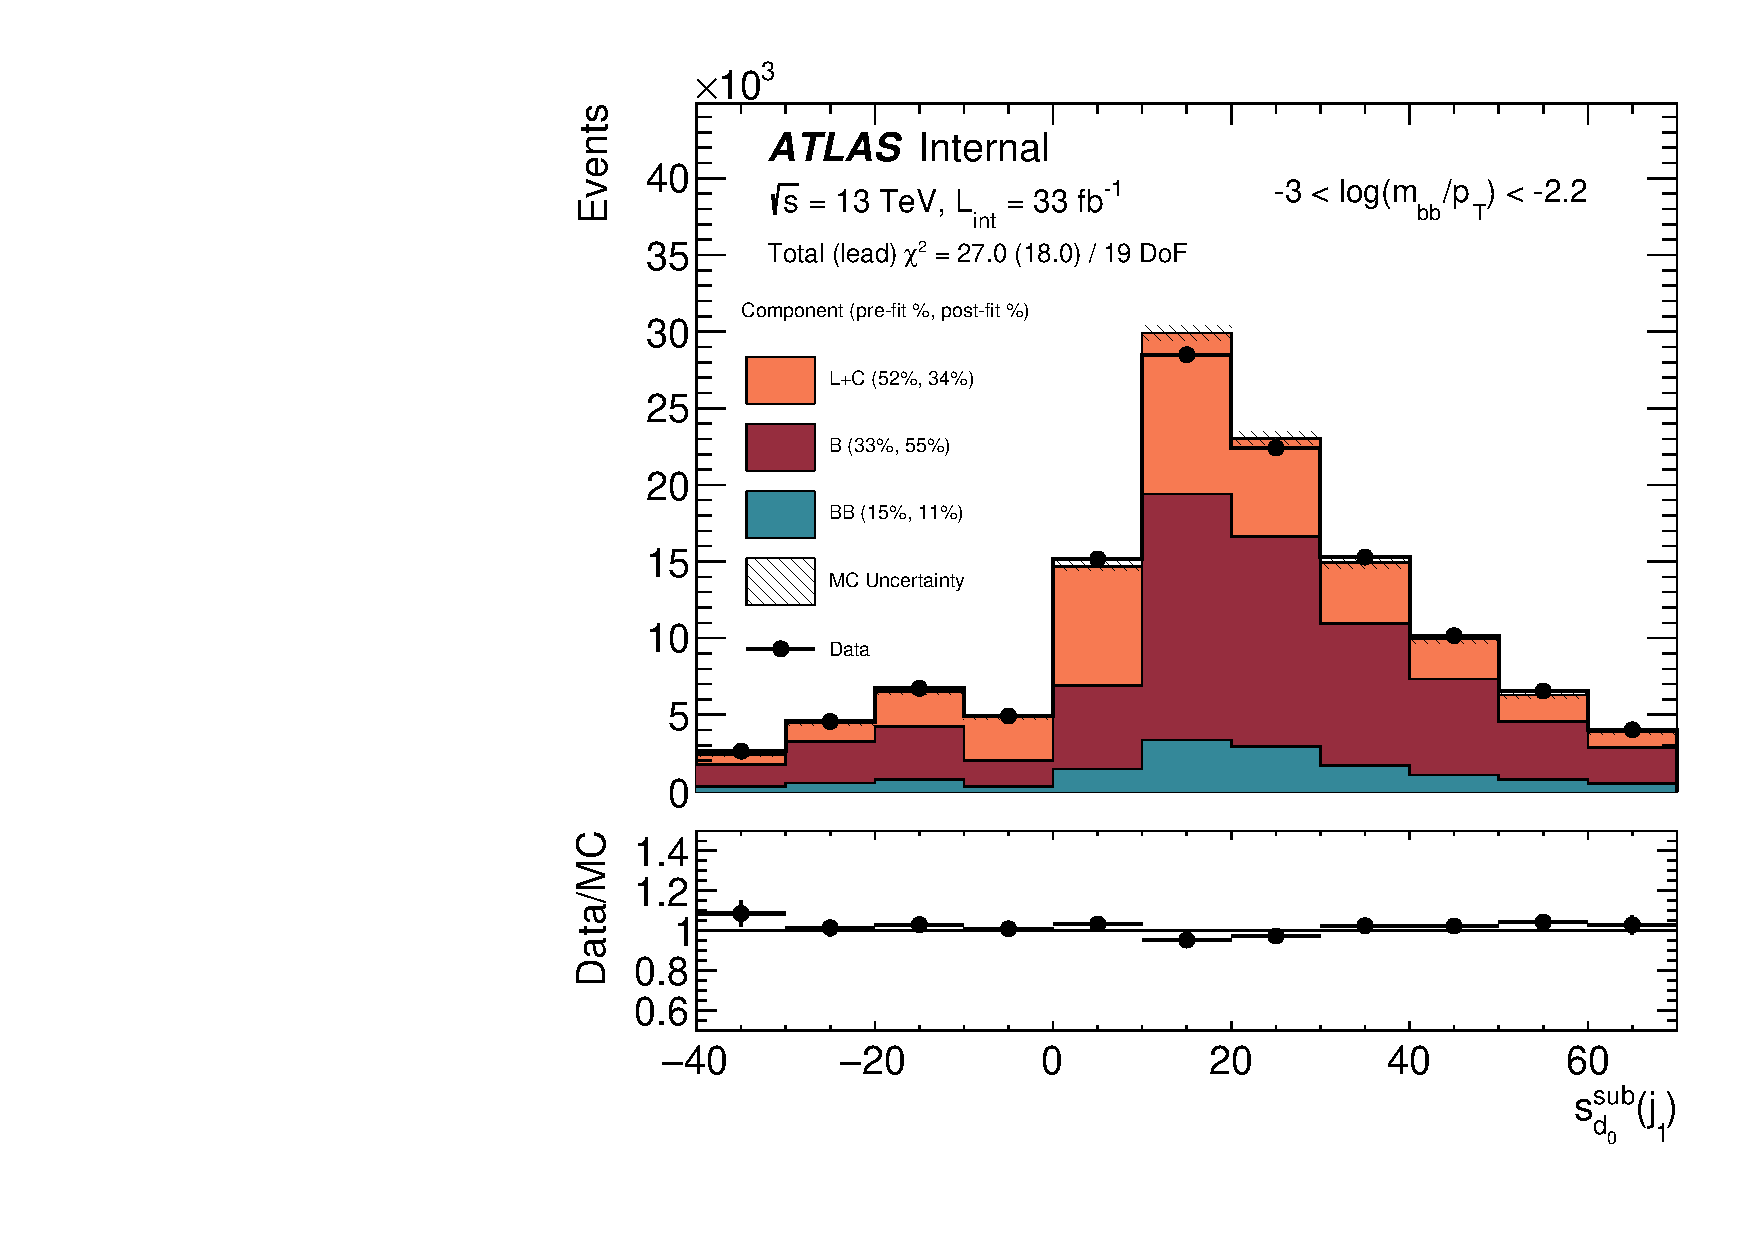
\includegraphics[width=0.45\textwidth]{figures/gbb/paperplots/Canv_Fit_M_LpT_INF_SpT_INF_coarse_x}
 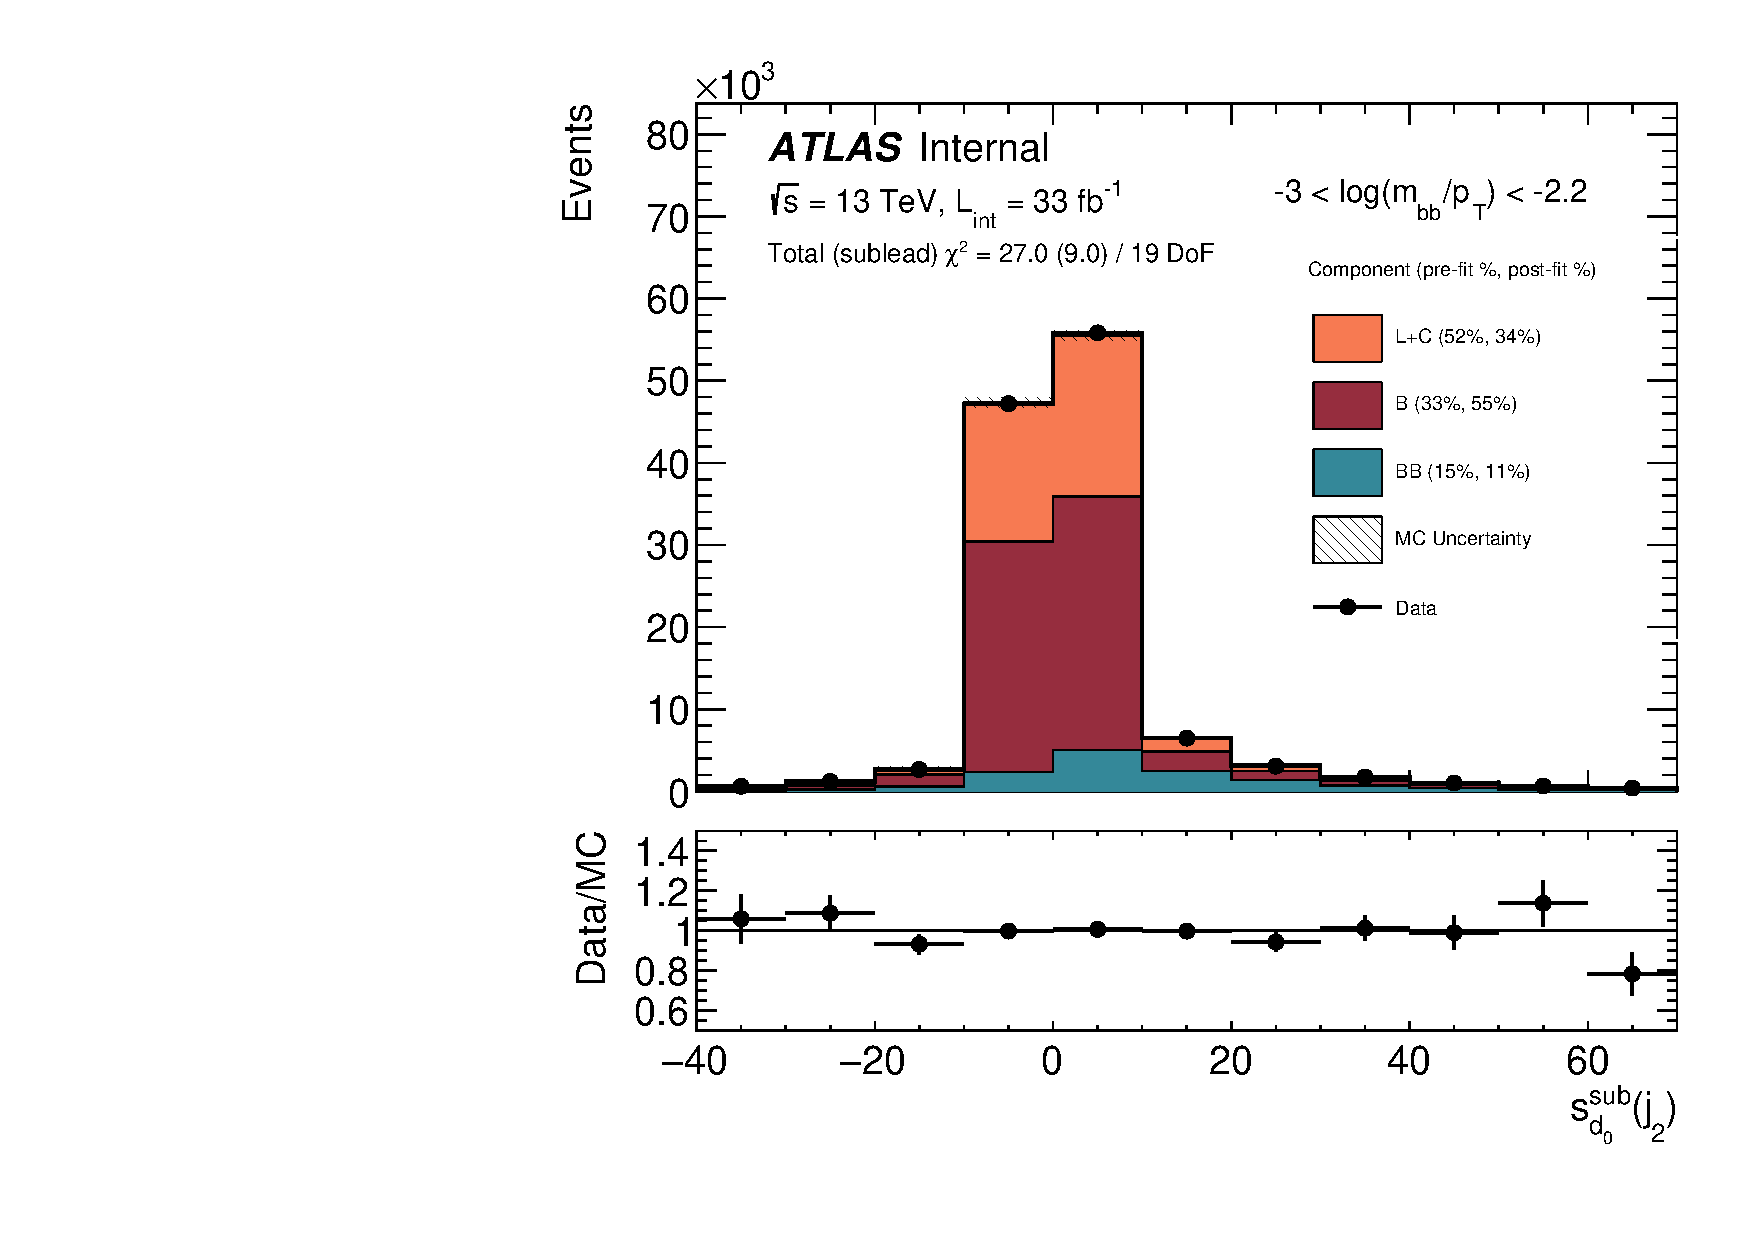
\includegraphics[width=0.45\textwidth]{figures/gbb/paperplots/Canv_Fit_b0_25_M_0_3_LpT_INF_SpT_INF_coarse_y}
 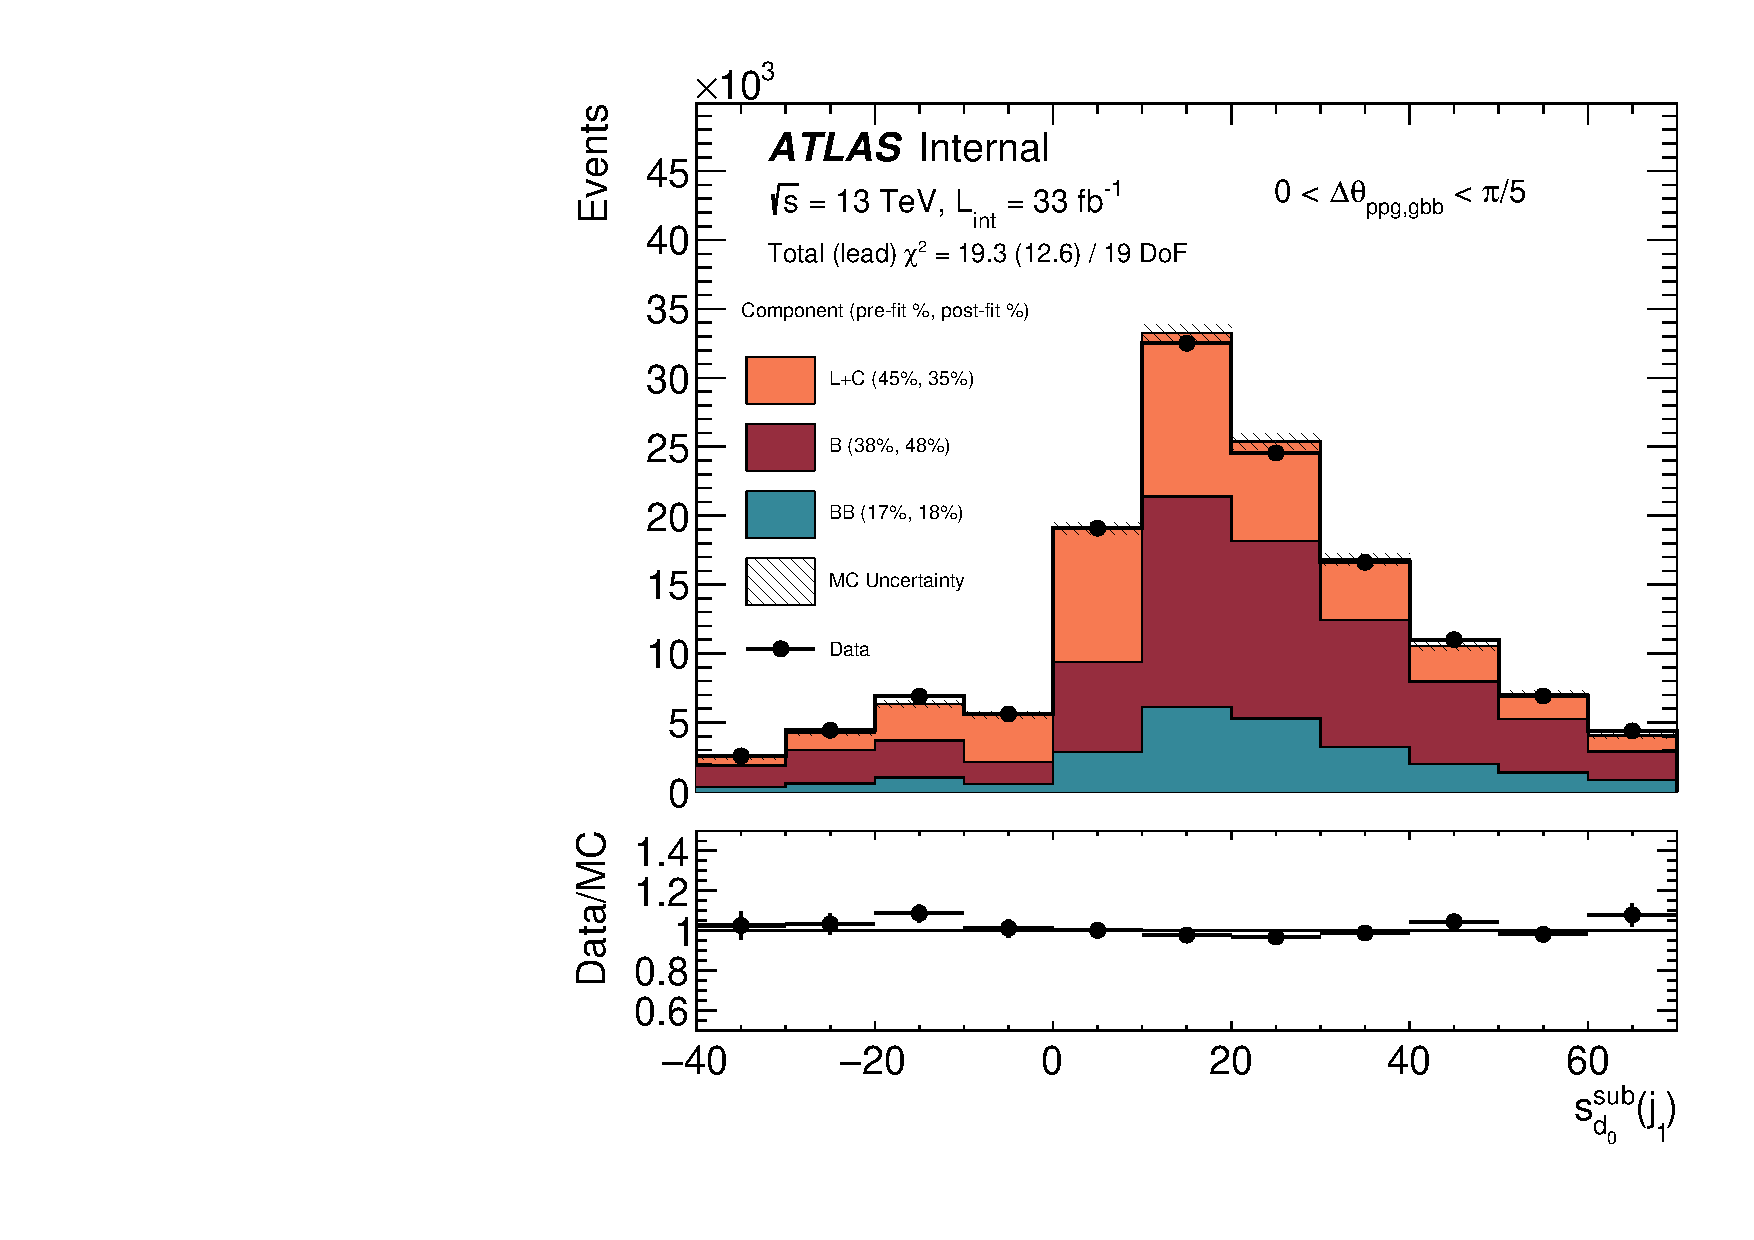
\includegraphics[width=0.45\textwidth]{figures/gbb/paperplots/Canv_Fit_dphi_LpT_INF_SpT_INF_coarse_x}
 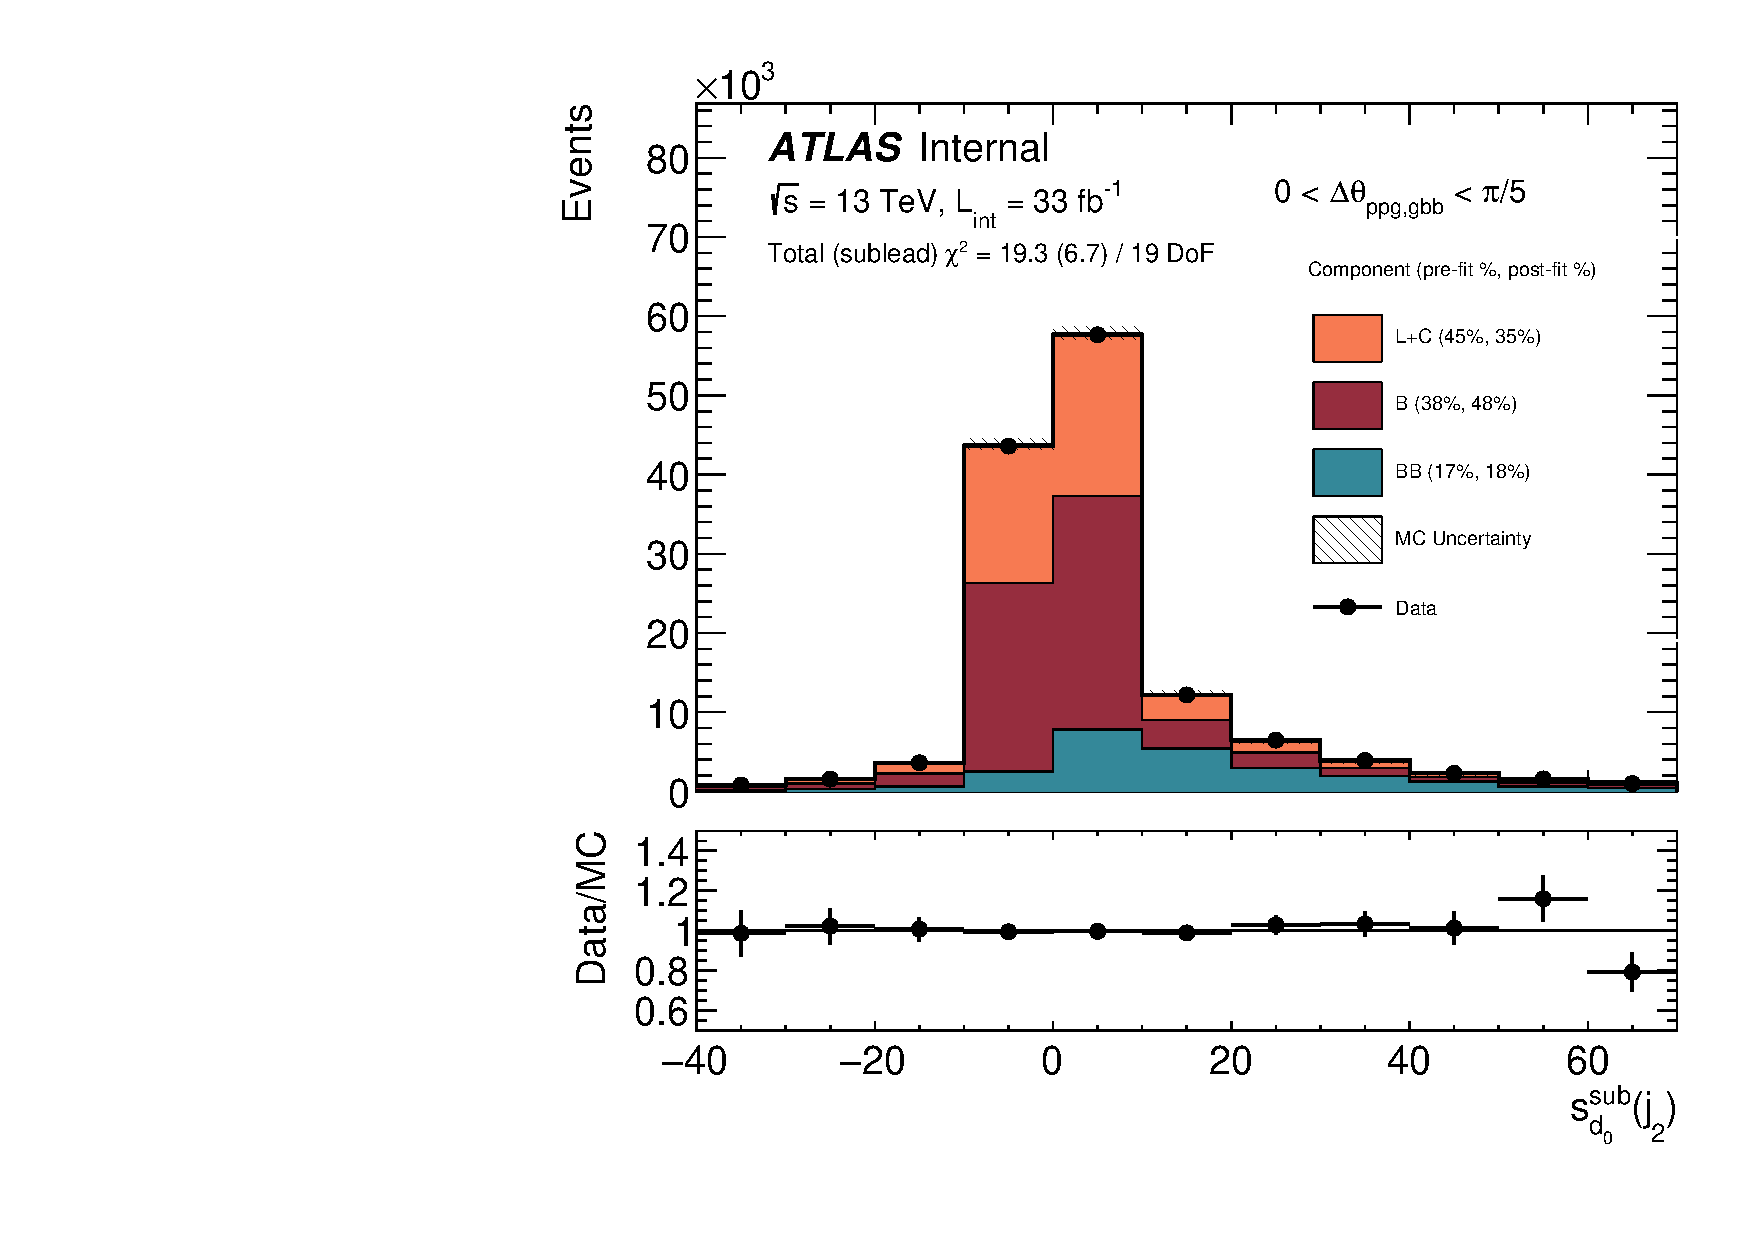
\includegraphics[width=0.45\textwidth]{figures/gbb/paperplots/Canv_Fit_b0_25_dphi_0_3_LpT_INF_SpT_INF_coarse_y}
\caption{Example of post-fit \subsdzero distributions of the leading (left) and sub-leading (right) track jets in bin of \drbb (first row), \zpt (second row), \mpt (third row) and \dphi (fourth row). Error bars only include statistical uncertainties.}
  \label{fig:fit-example}
\end{figure}

\begin{figure}[htbp]
  \centering
  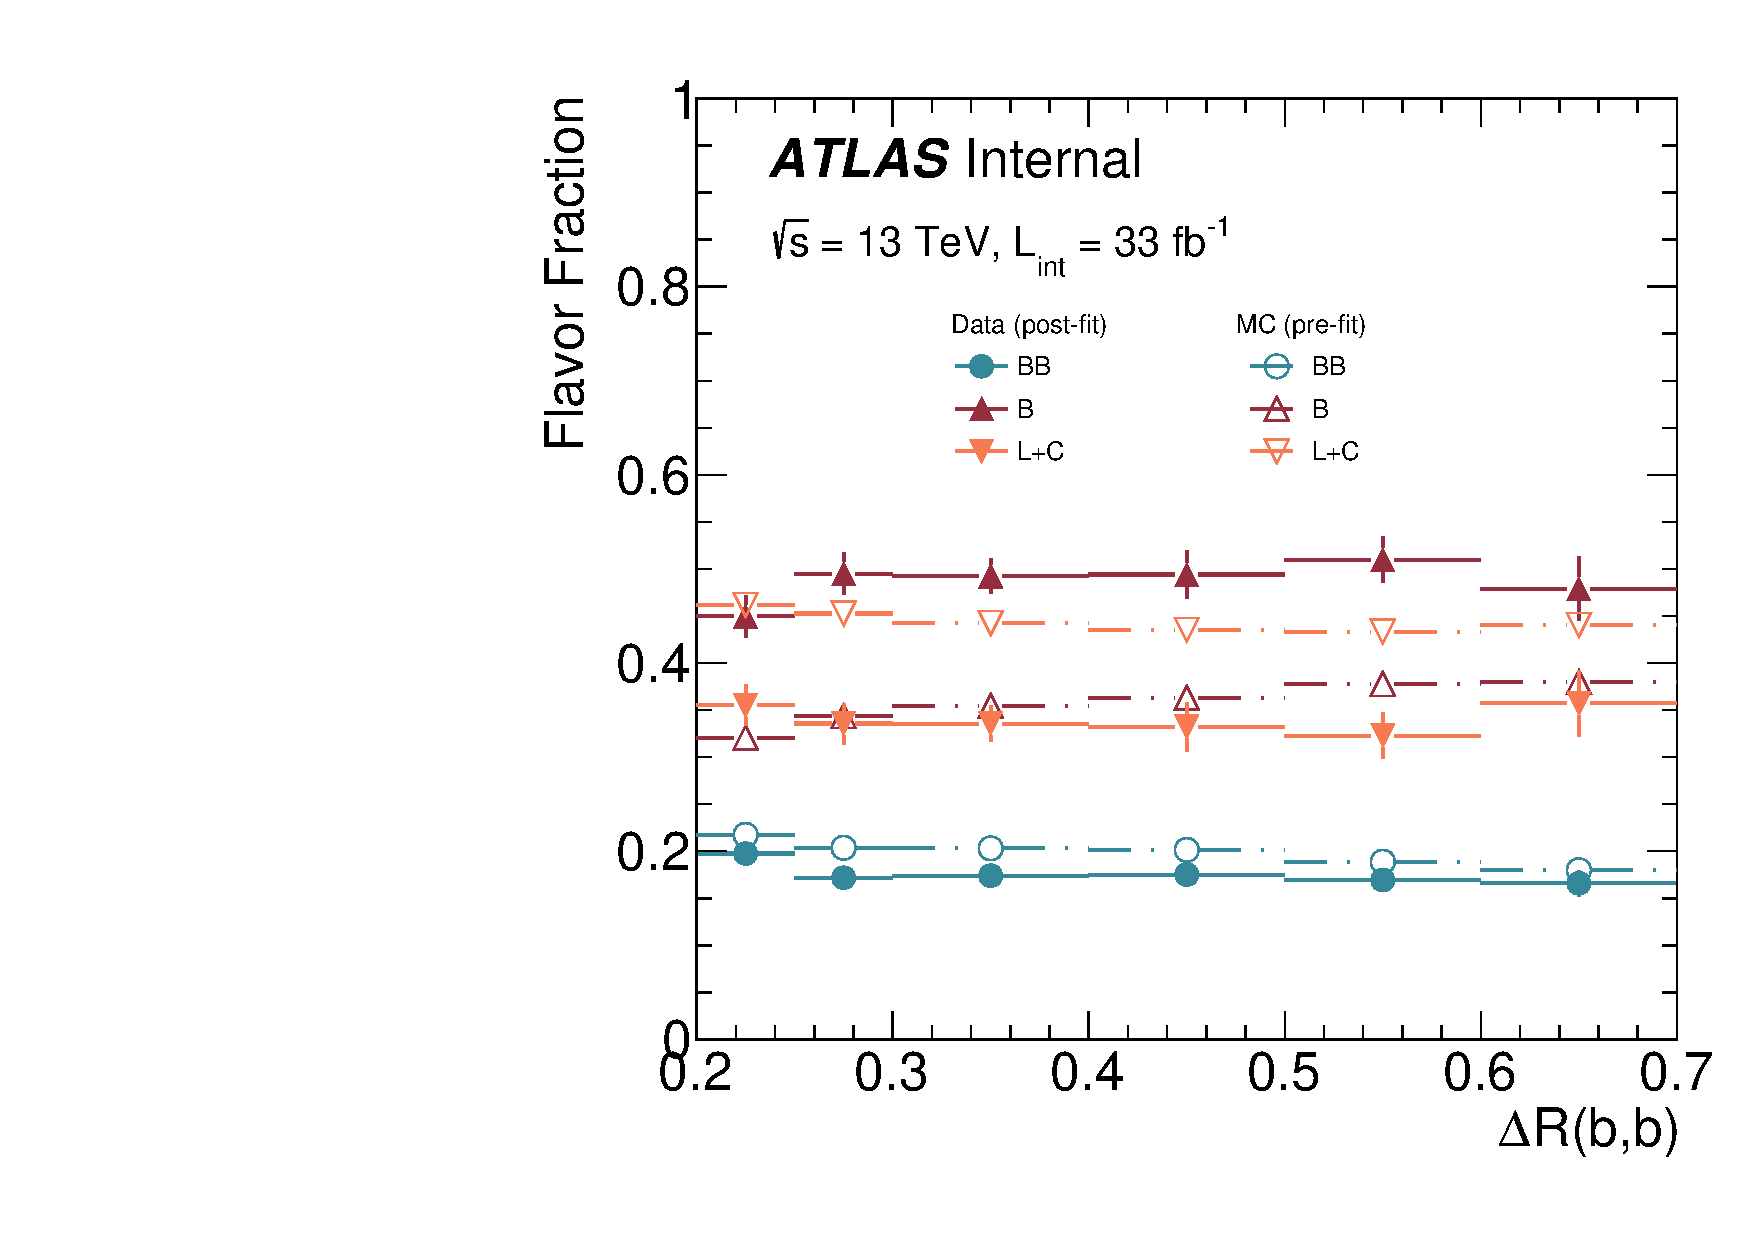
\includegraphics[width=0.45\textwidth]{figures/gbb/paperplots/Canv_dR_FracDataMC}
  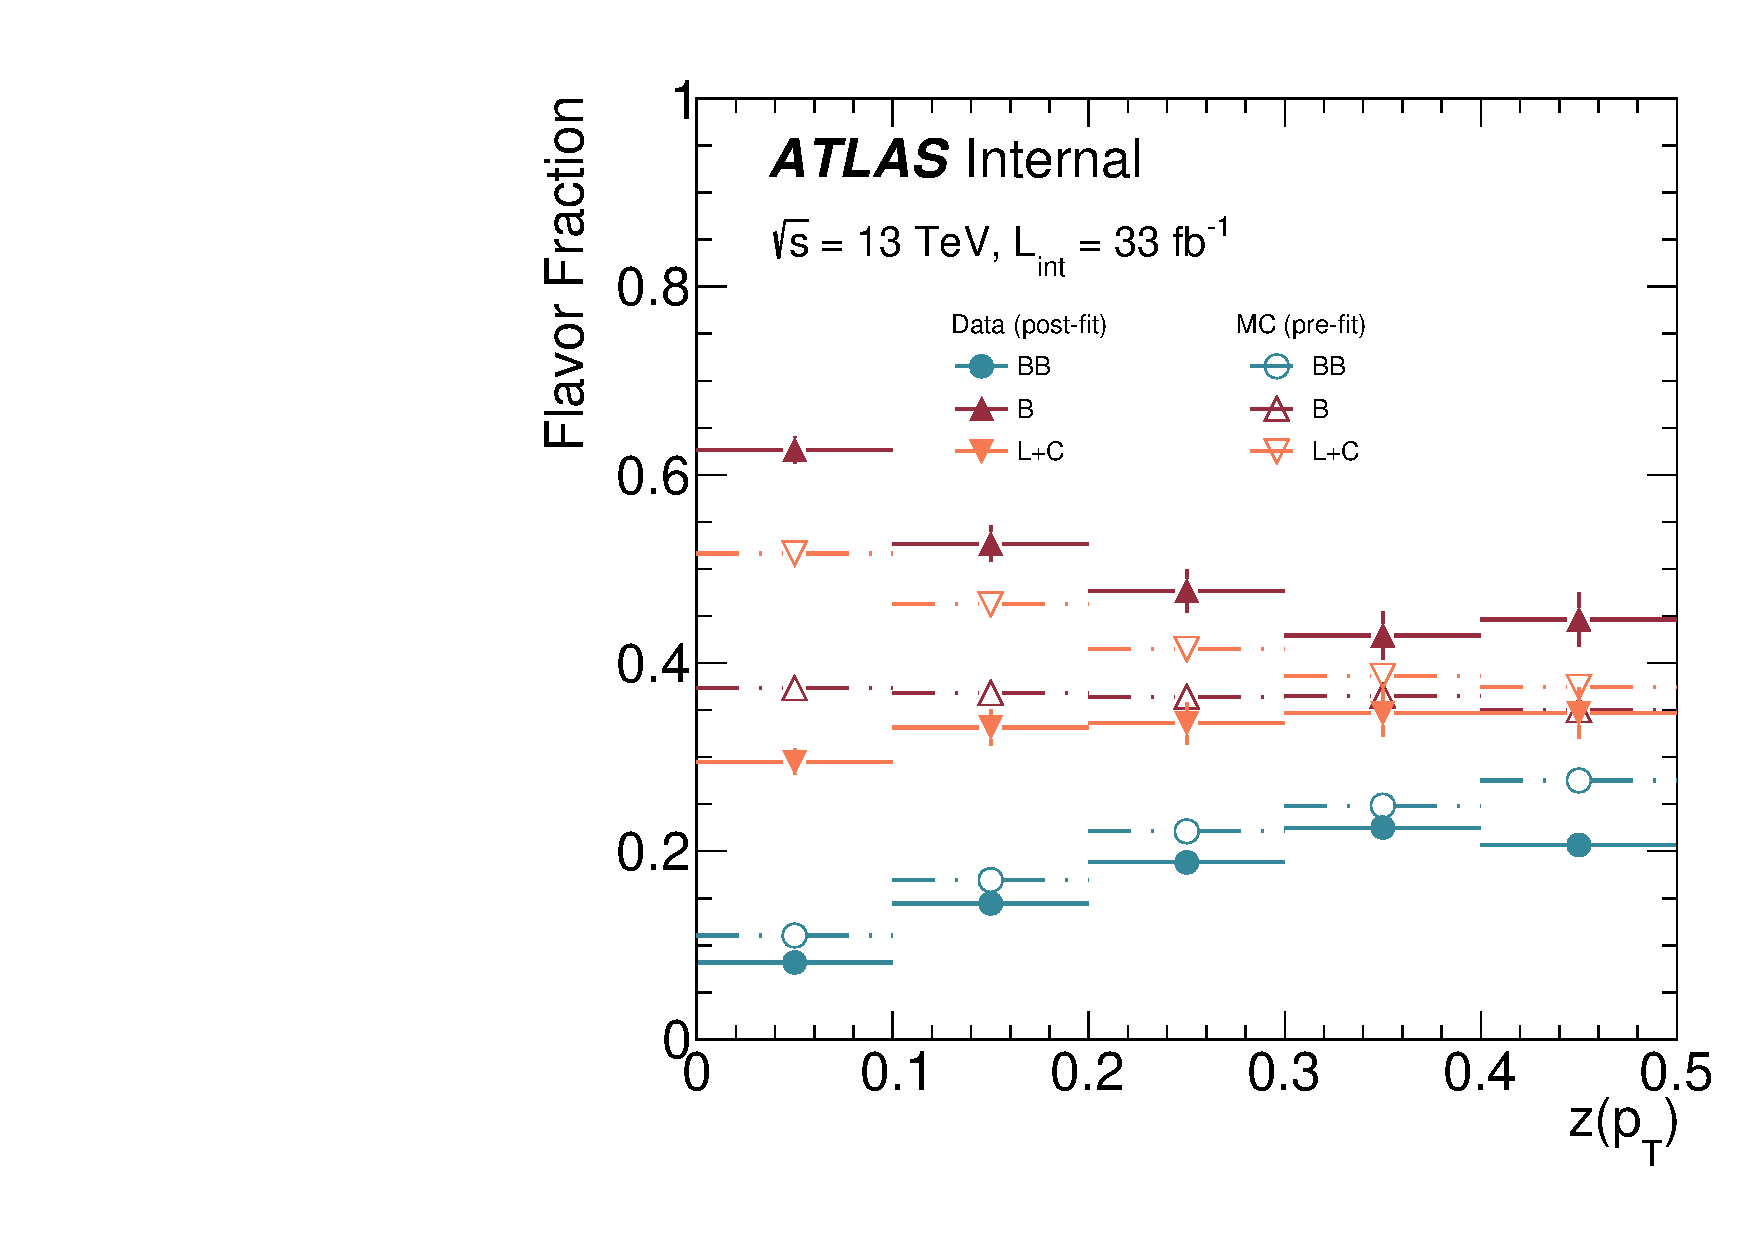
\includegraphics[width=0.45\textwidth]{figures/gbb/paperplots/Canv_ZpT_FracDataMC}
  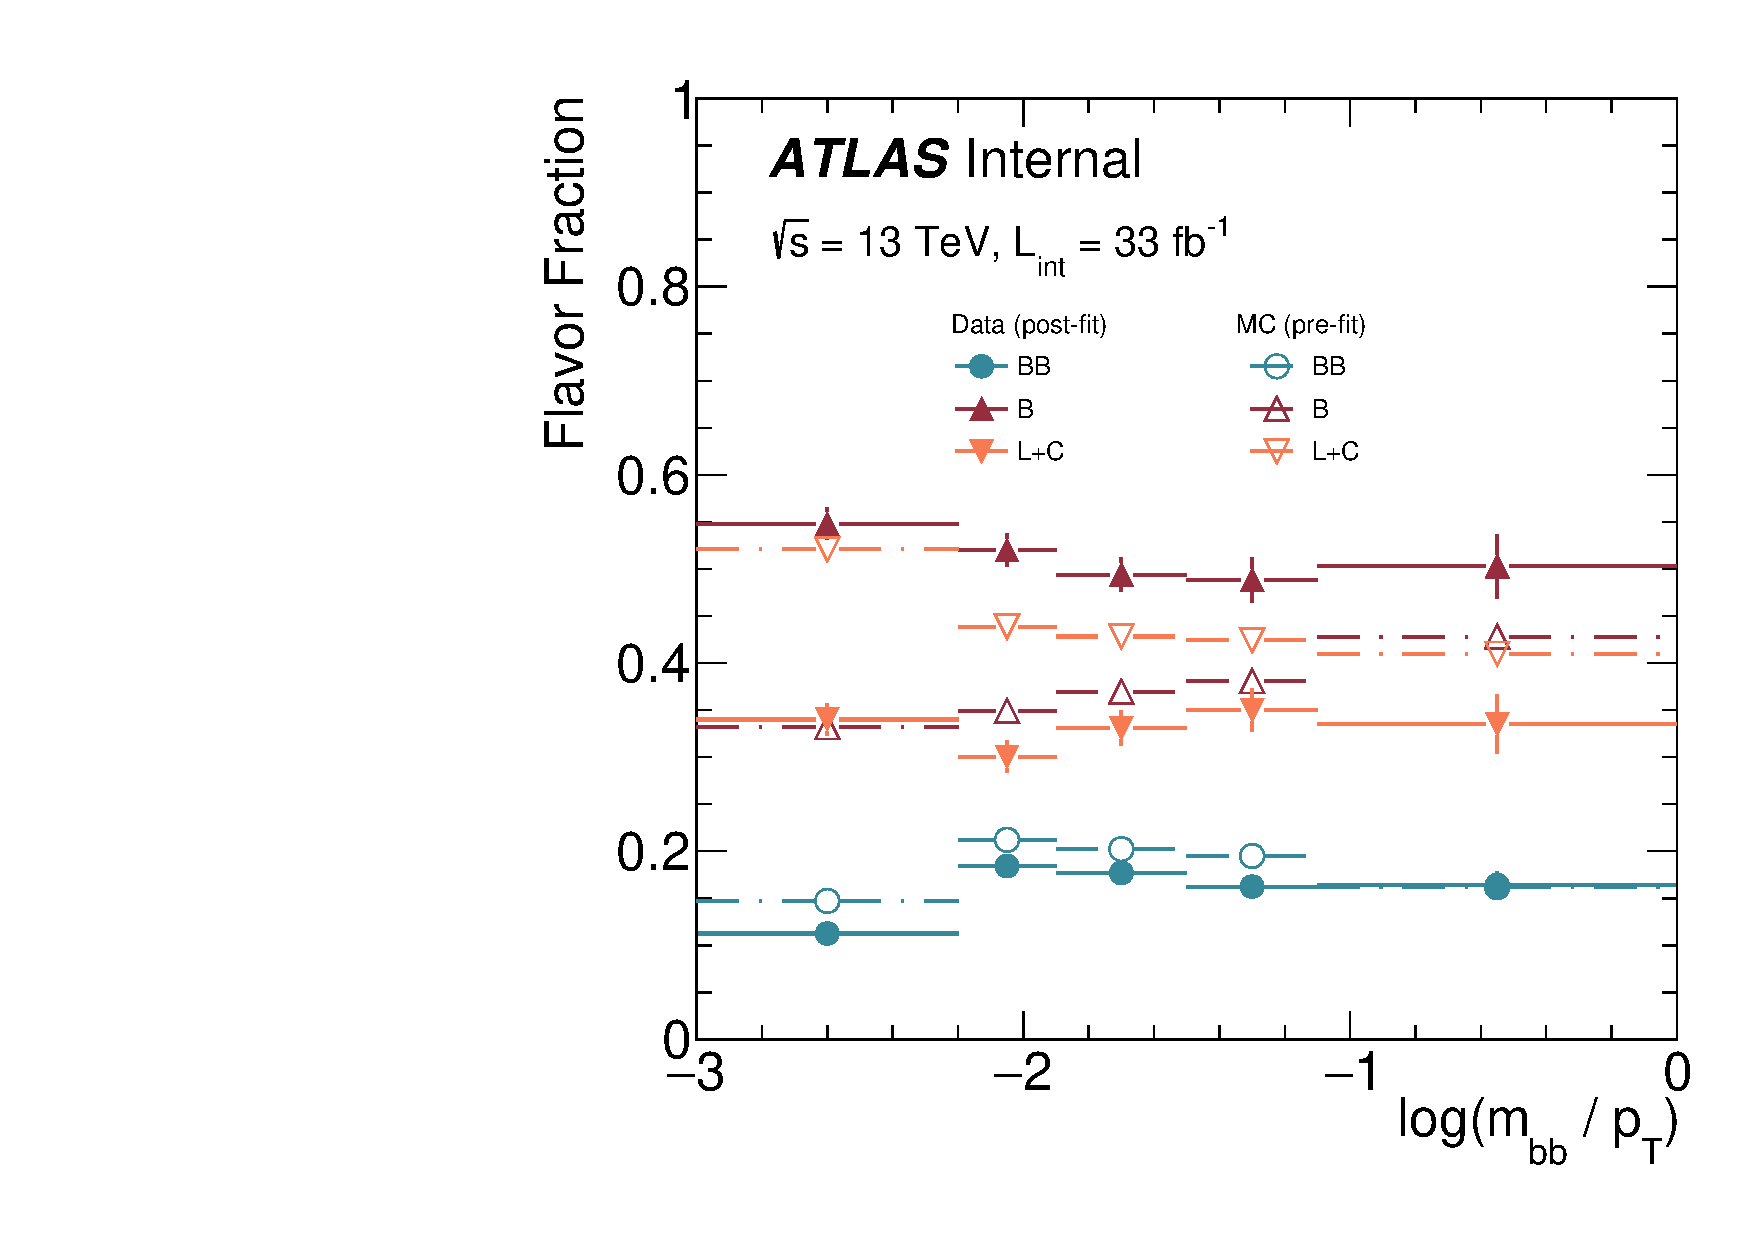
\includegraphics[width=0.45\textwidth]{figures/gbb/paperplots/Canv_fracmasspt_FracDataMC}       
  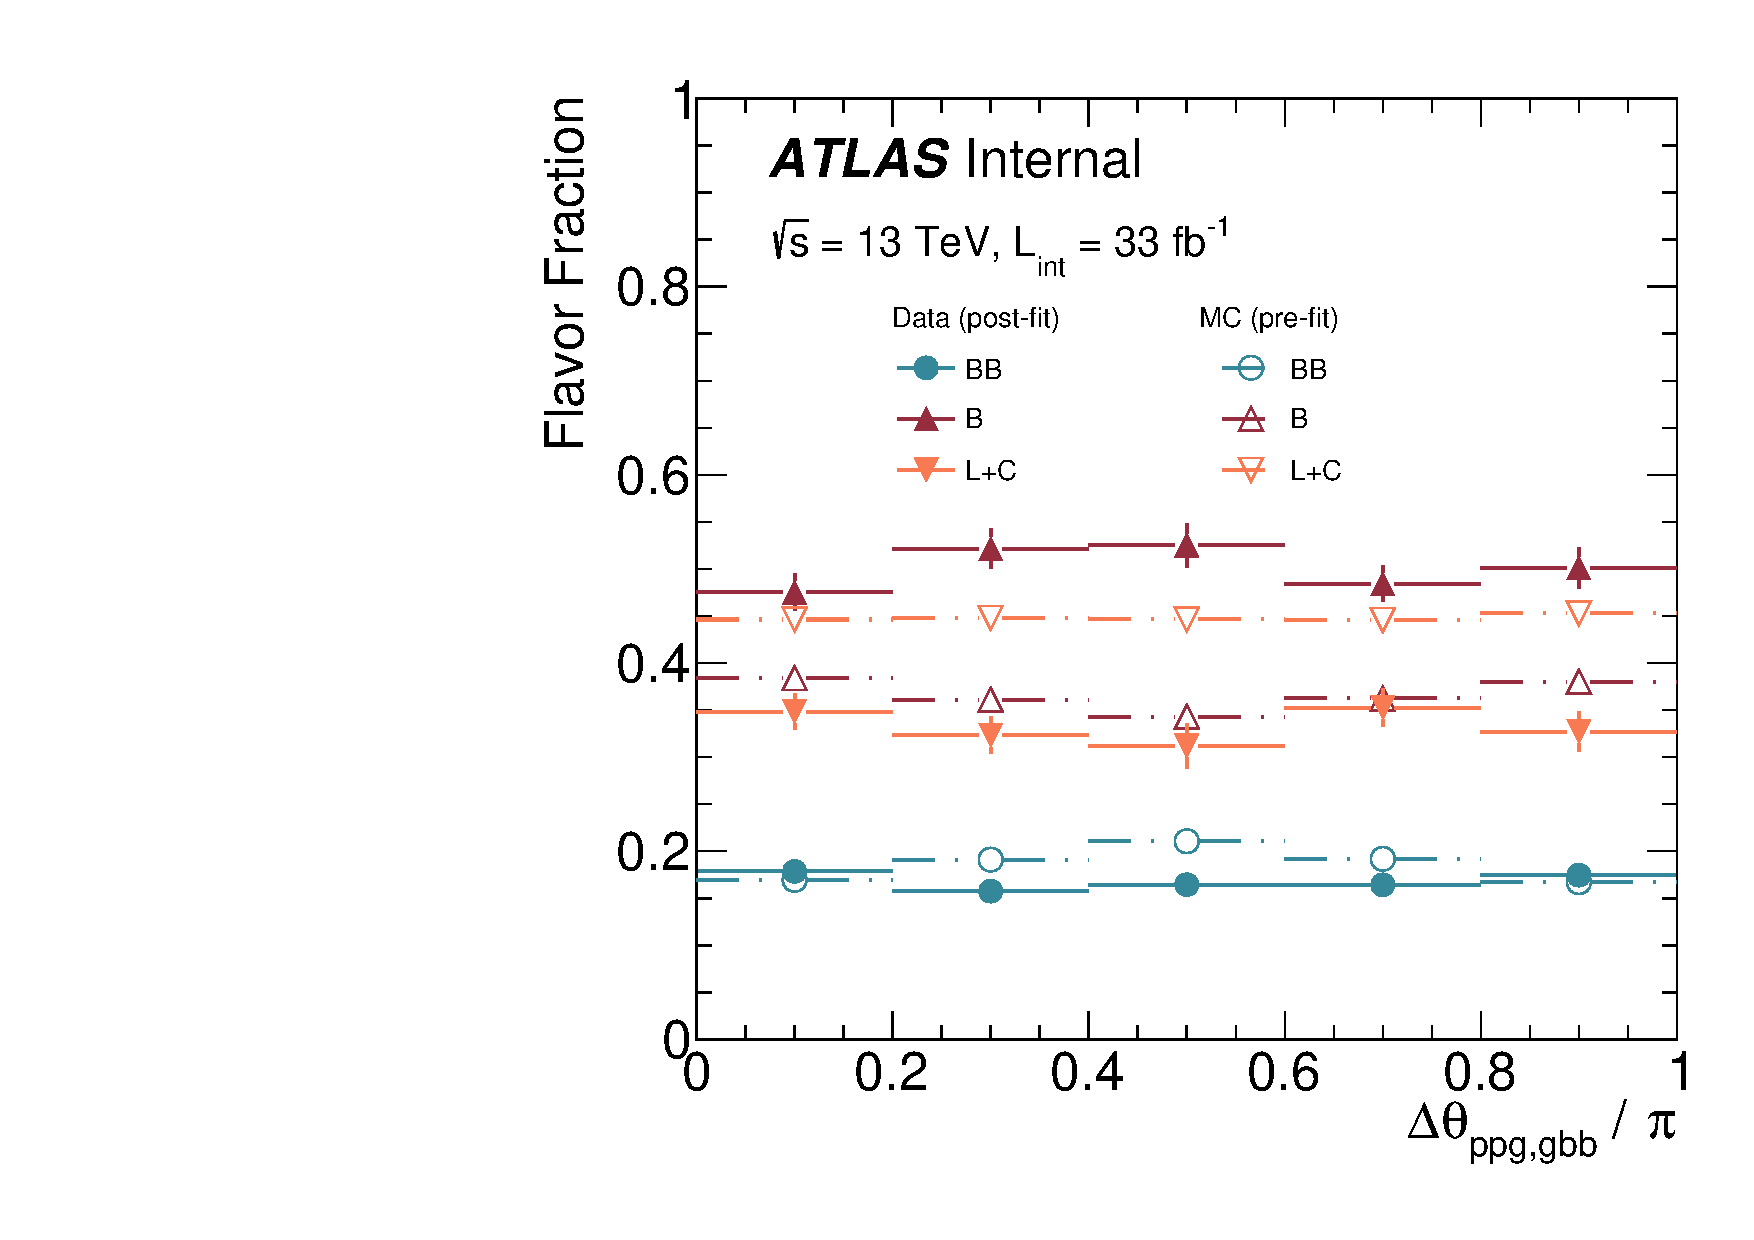
\includegraphics[width=0.45\textwidth]{figures/gbb/paperplots/Canv_dphi_FracDataMC}       
\caption{MC predicted (hollow) and fitted (solid) flavor fraction in bins of \drbb (top left), \zpt (top right), \mpt (bottom left) and \dphi (bottom right). The error bar is the quadrature sum of the uncertainty derived from fit range systematics and fit statistics as defined in Sec.\ref{sec:gbb-sub_systematics} }
  \label{fig:gbb-fitfrac}
\end{figure}


\begin{figure}[htbp]
  \centering
 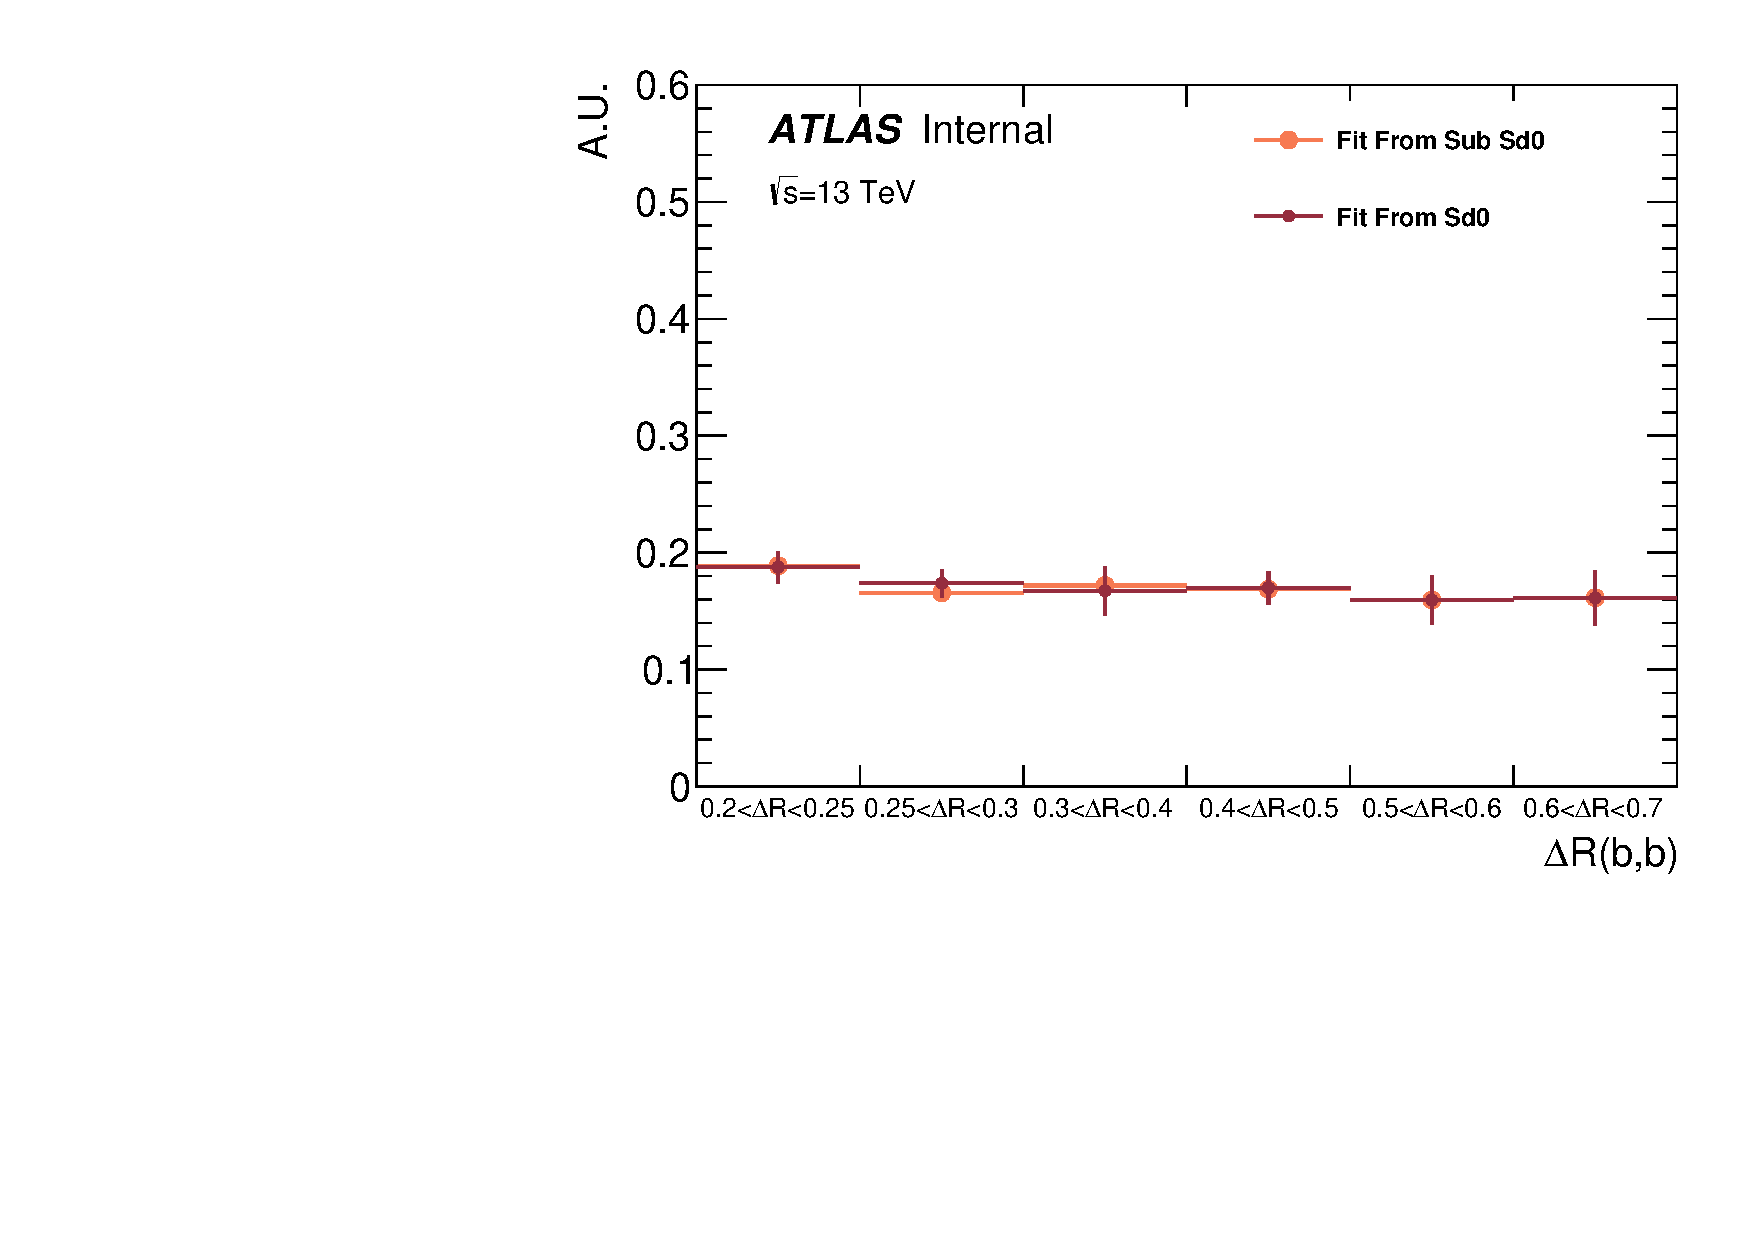
\includegraphics[width=0.45\textwidth]{figures/gbb/Sub_Sd0_Fits/Canv_dR_leadCrossCheck.pdf}
 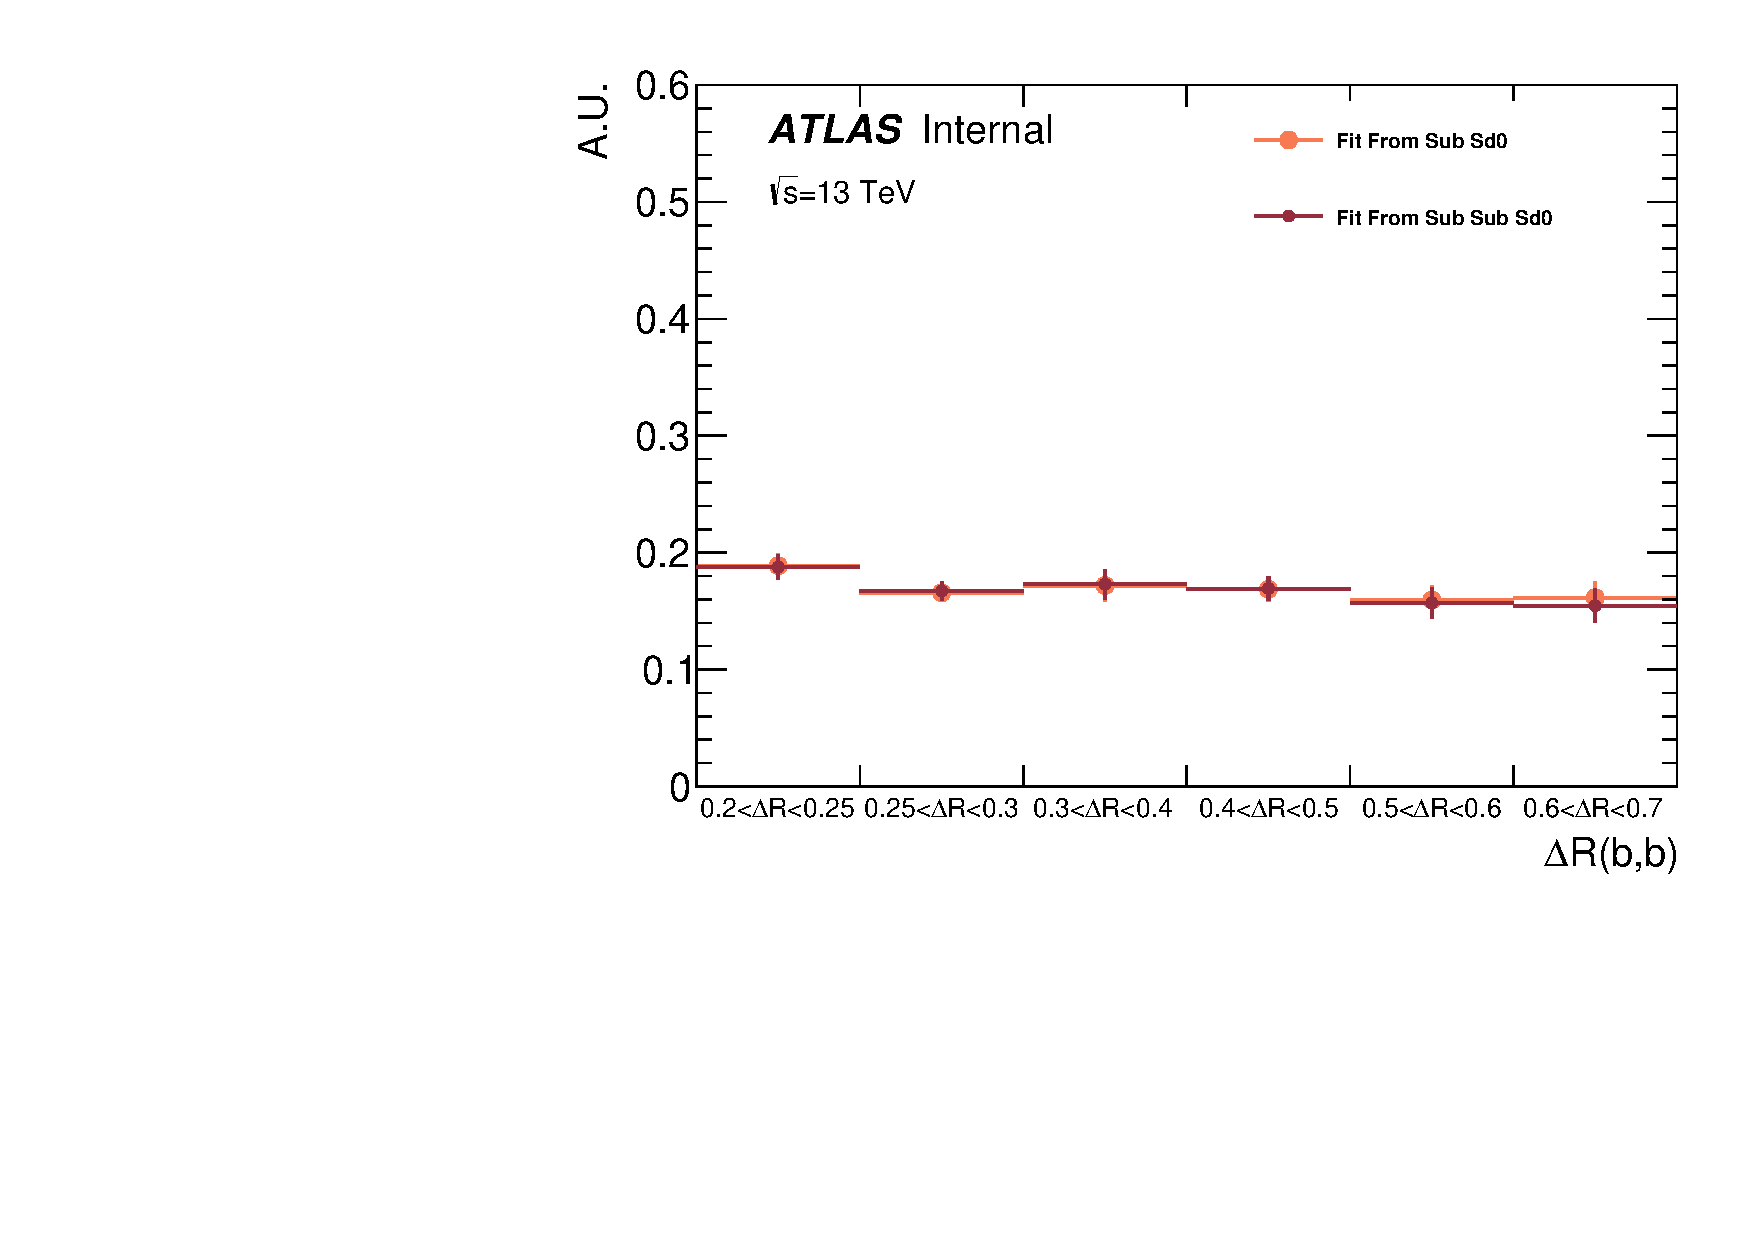
\includegraphics[width=0.45\textwidth]{figures/gbb/Sub_Sd0_Fits/Canv_dR_subsubCrossCheck.pdf}\\
 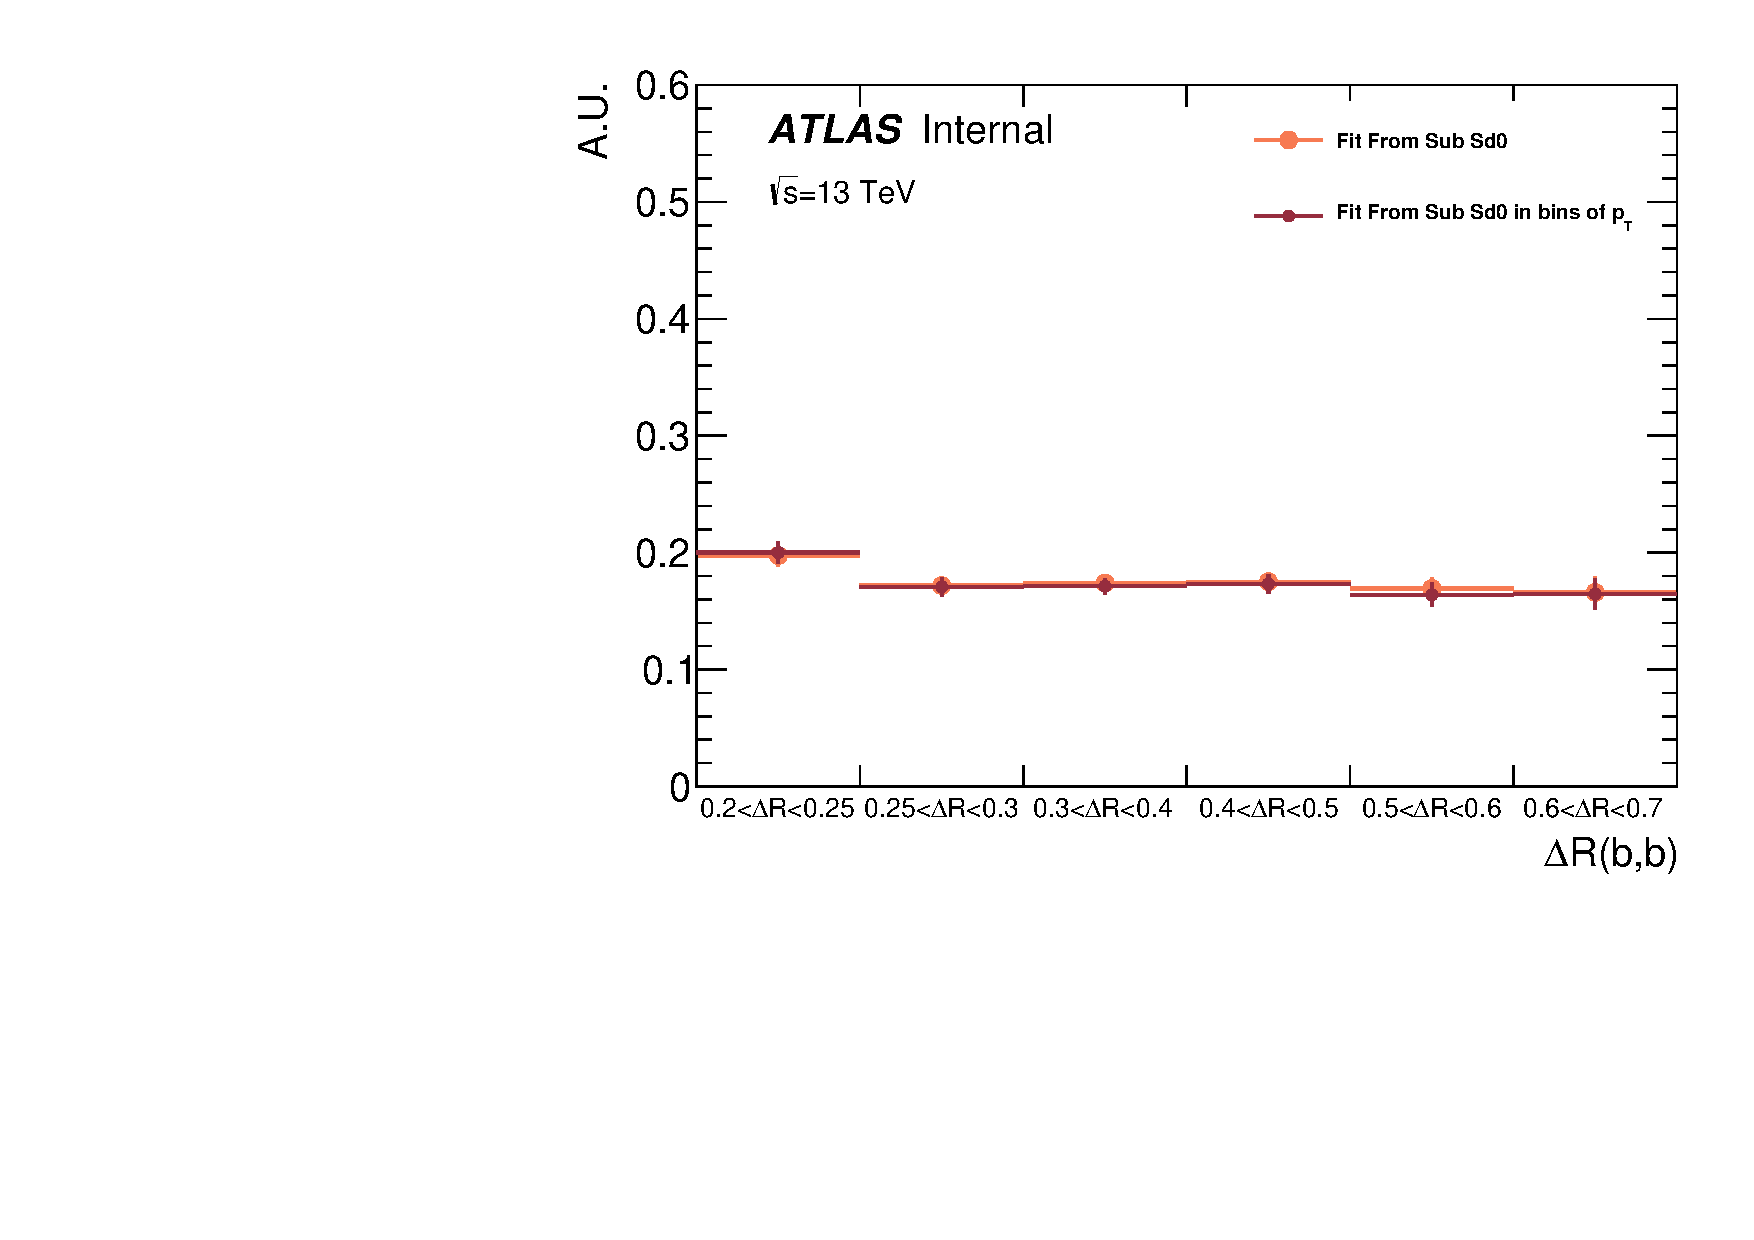
\includegraphics[width=0.45\textwidth]{figures/gbb/Sub_Sd0_Fits/Canv_dR_ptbinCrossCheck.pdf}
 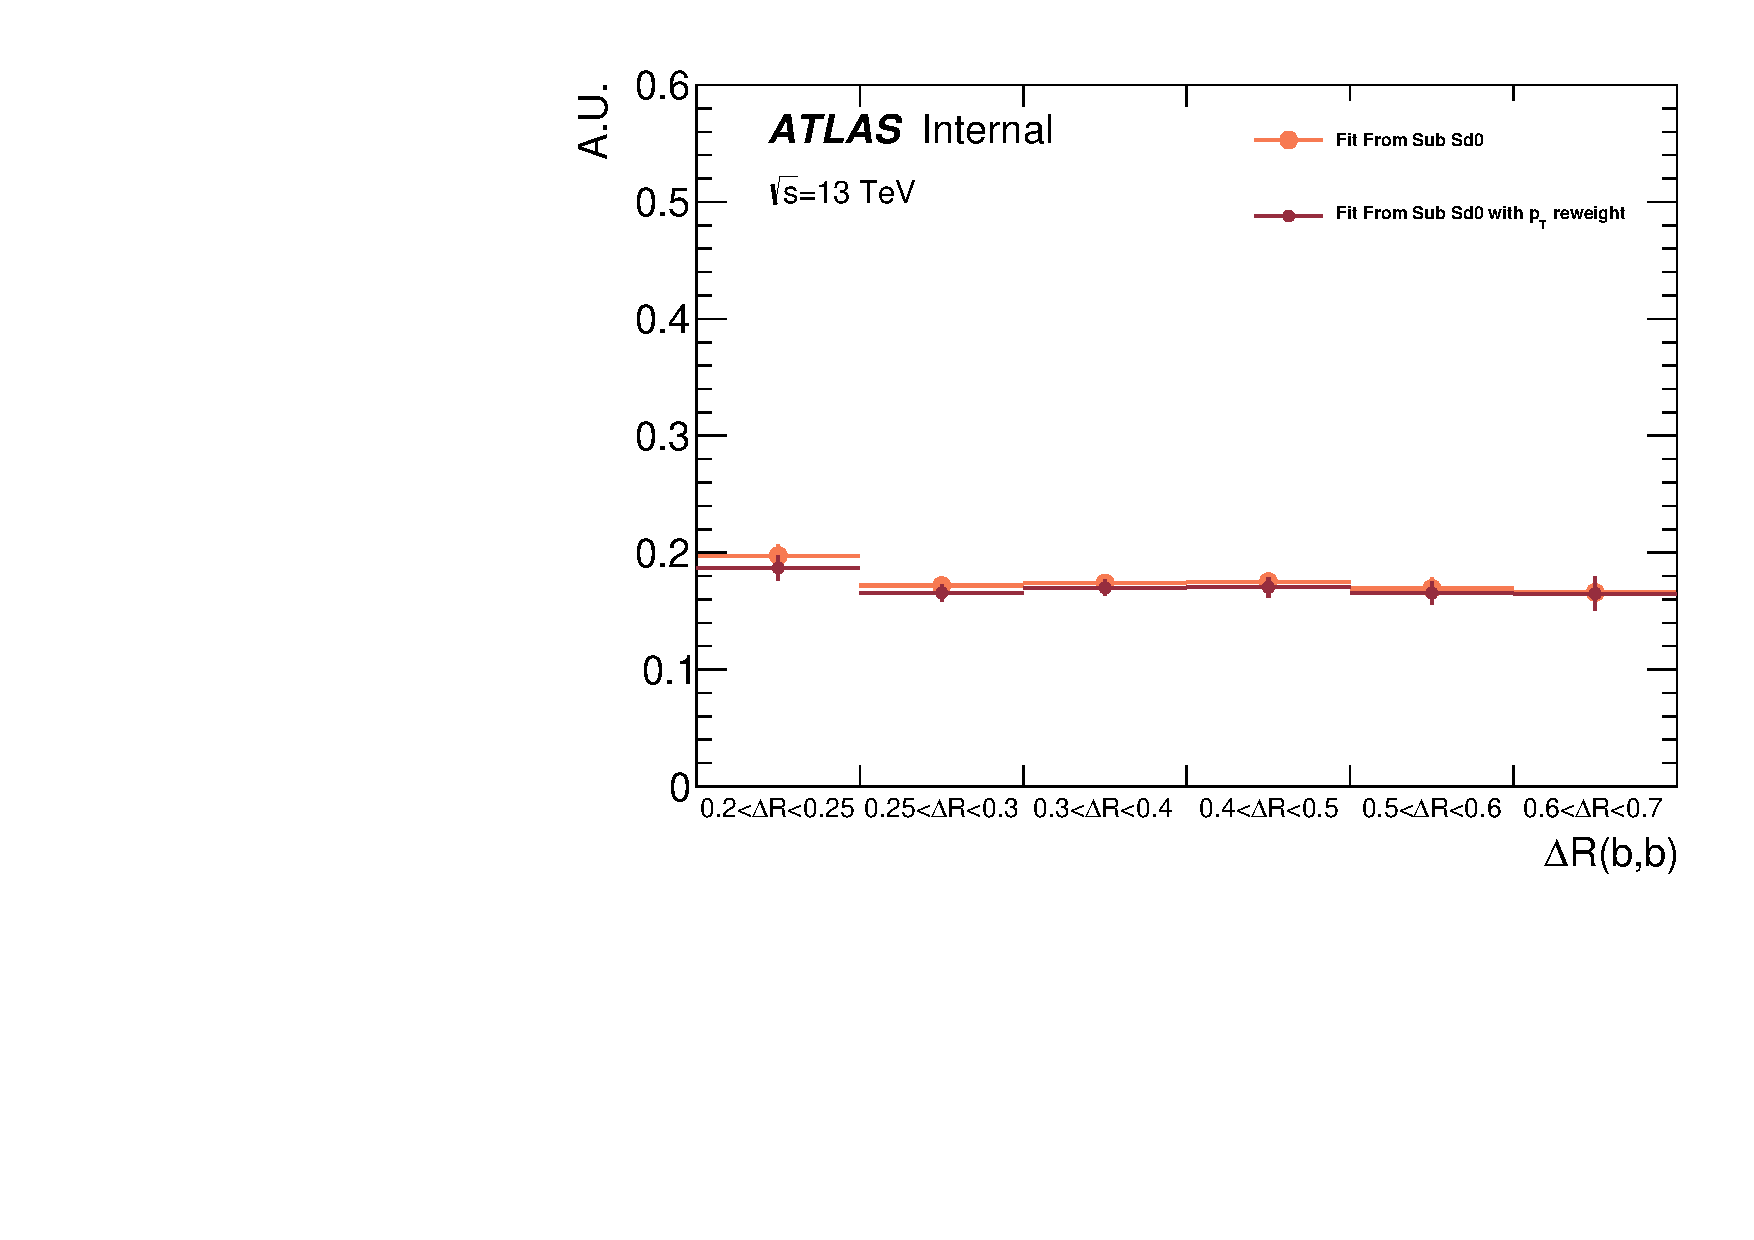
\includegraphics[width=0.45\textwidth]{figures/gbb/Sub_Sd0_Fits/Canv_dR_noreweightCrossCheck.pdf}\\
\caption{Comparison of flavor fractions fitted (1) using \subsdzero and \sdzero (top left), (2) using \subsdzero and \subsubsdzero (top right), (3) using inclusive and $p_T$ parameterized templates (bottom left) and (4) with and without track jet kinematic re-weighting in bins of \drbb}
  \label{fig:dR-fitfrac-crosscheck}
\end{figure}

\begin{figure}[htbp]
  \centering
 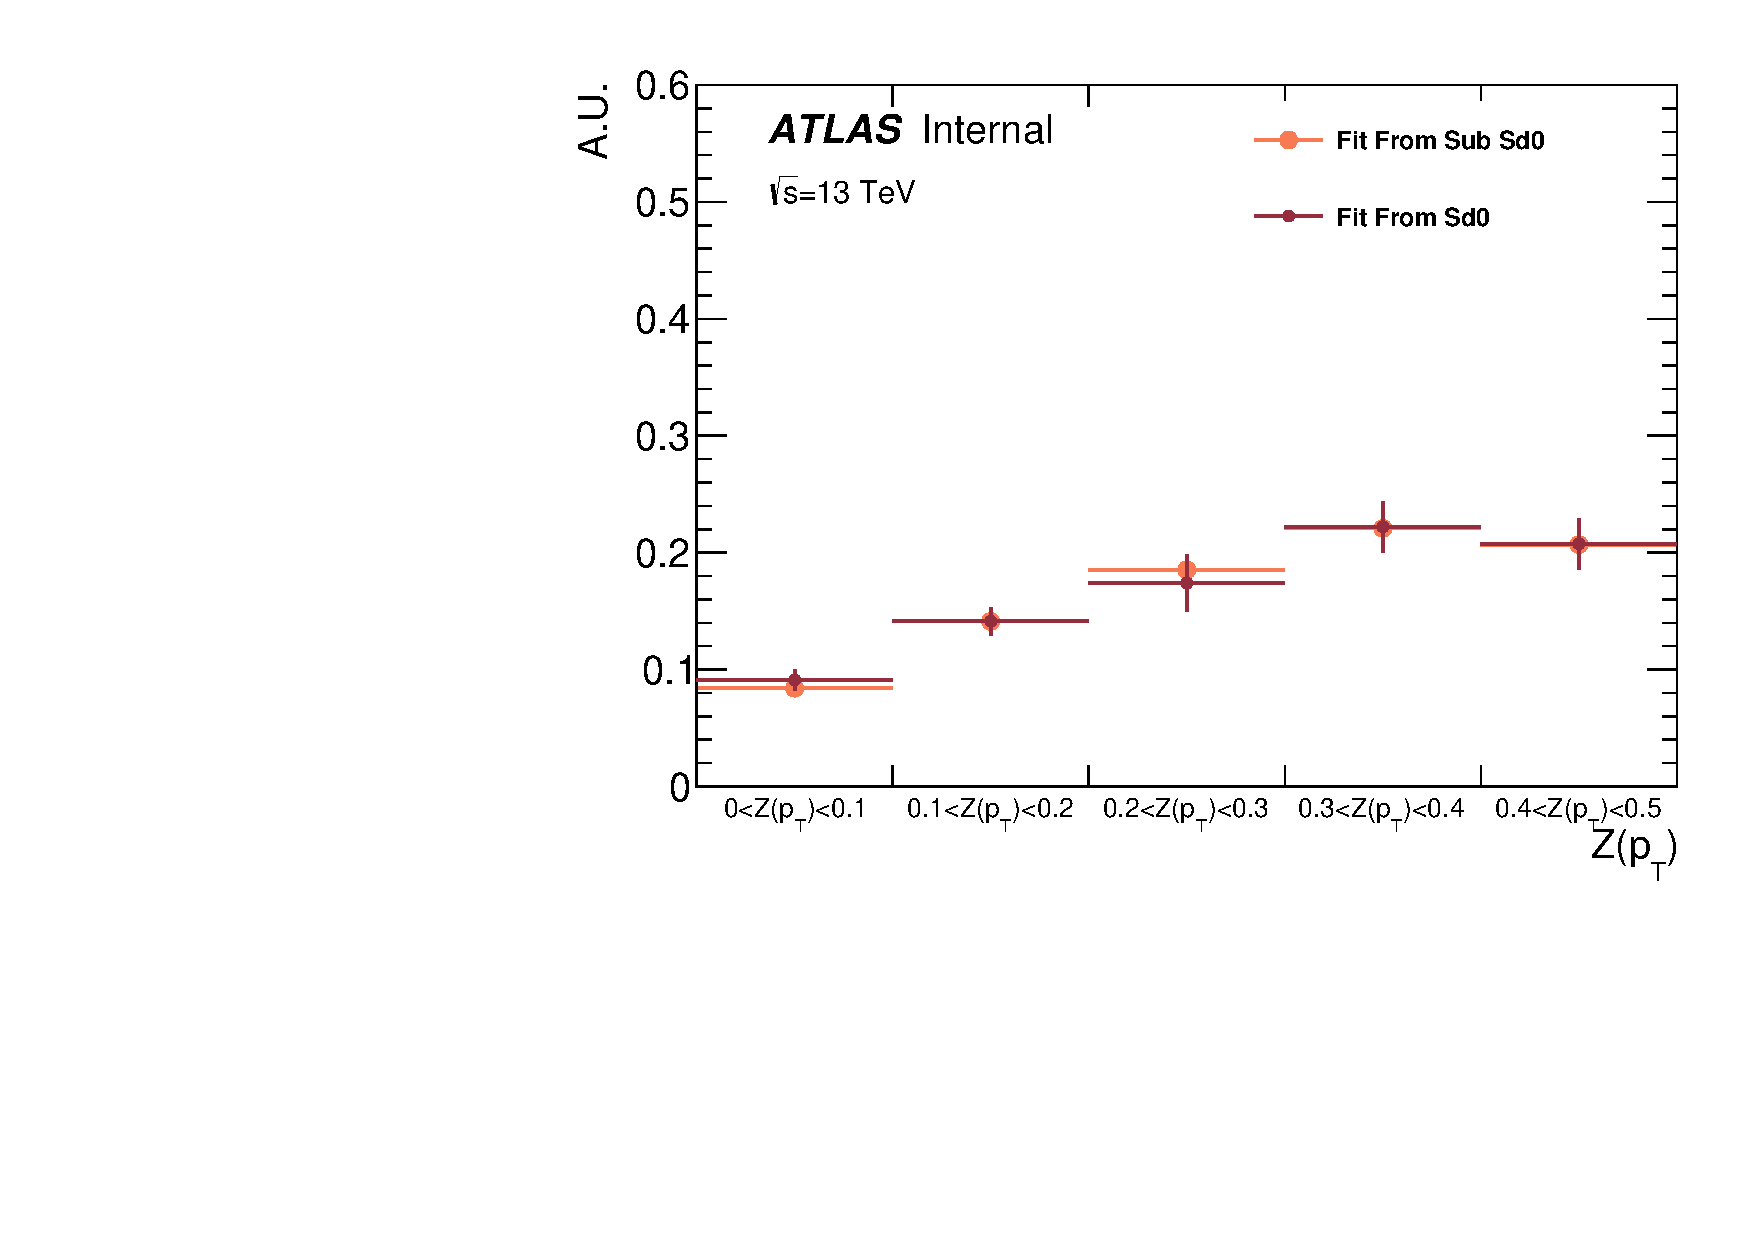
\includegraphics[width=0.45\textwidth]{figures/gbb/Sub_Sd0_Fits/Canv_ZpT_leadCrossCheck.pdf}
 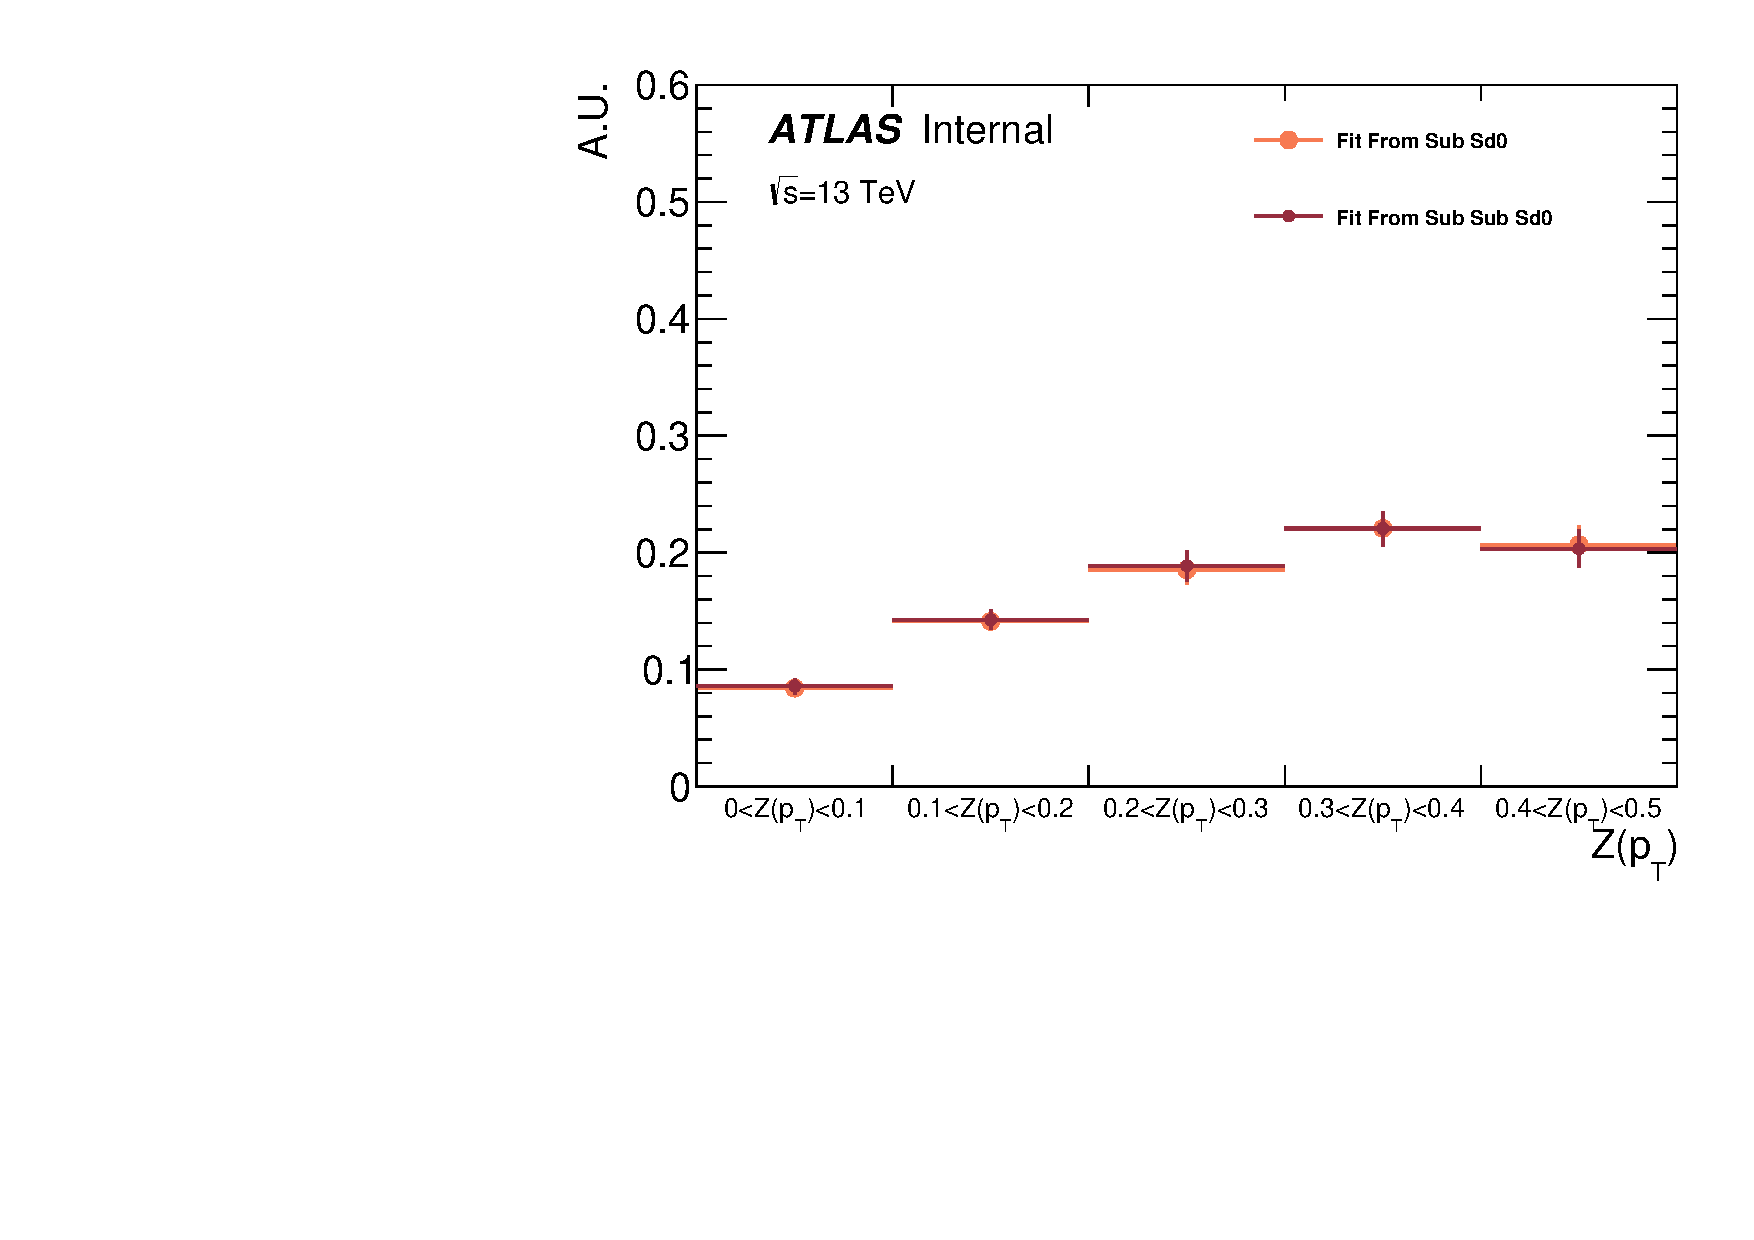
\includegraphics[width=0.45\textwidth]{figures/gbb/Sub_Sd0_Fits/Canv_ZpT_subsubCrossCheck.pdf}\\
 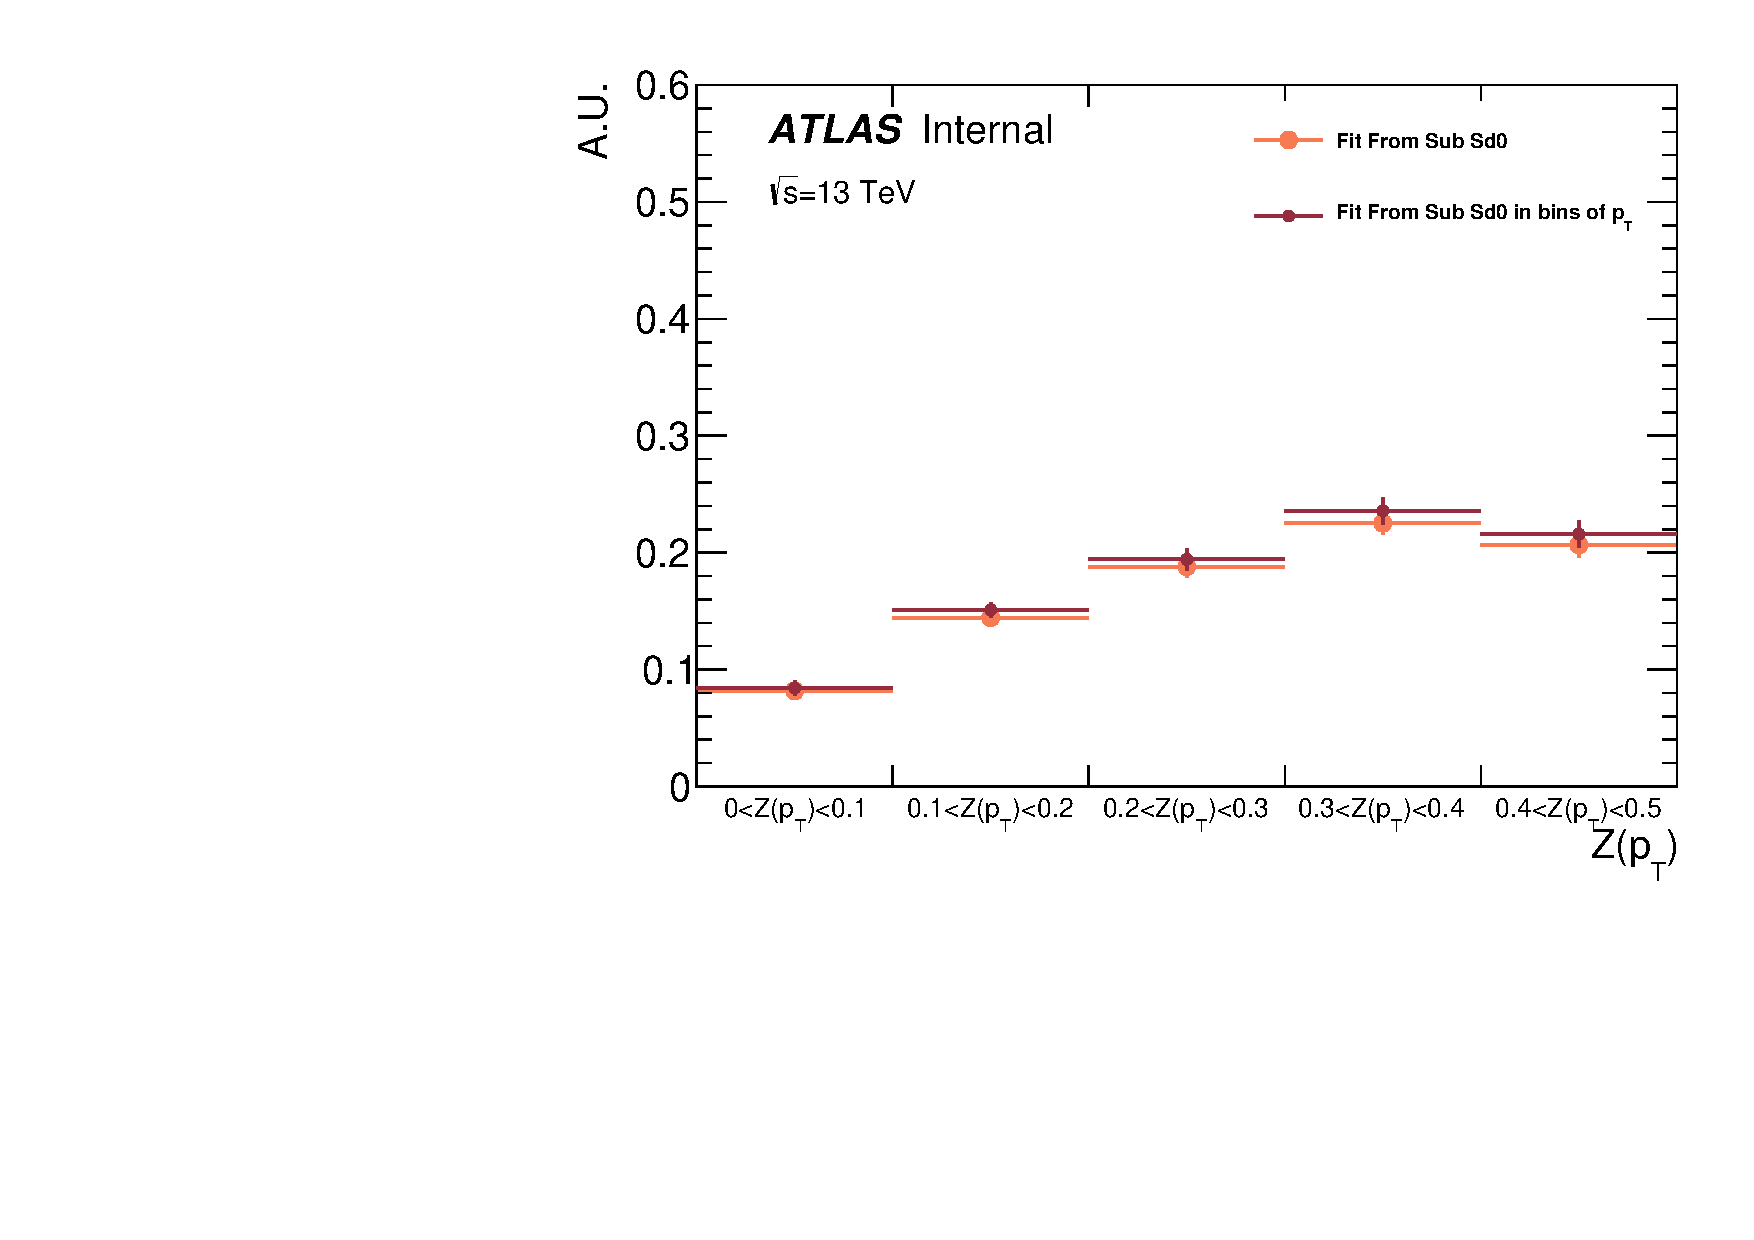
\includegraphics[width=0.45\textwidth]{figures/gbb/Sub_Sd0_Fits/Canv_ZpT_ptbinCrossCheck.pdf}
 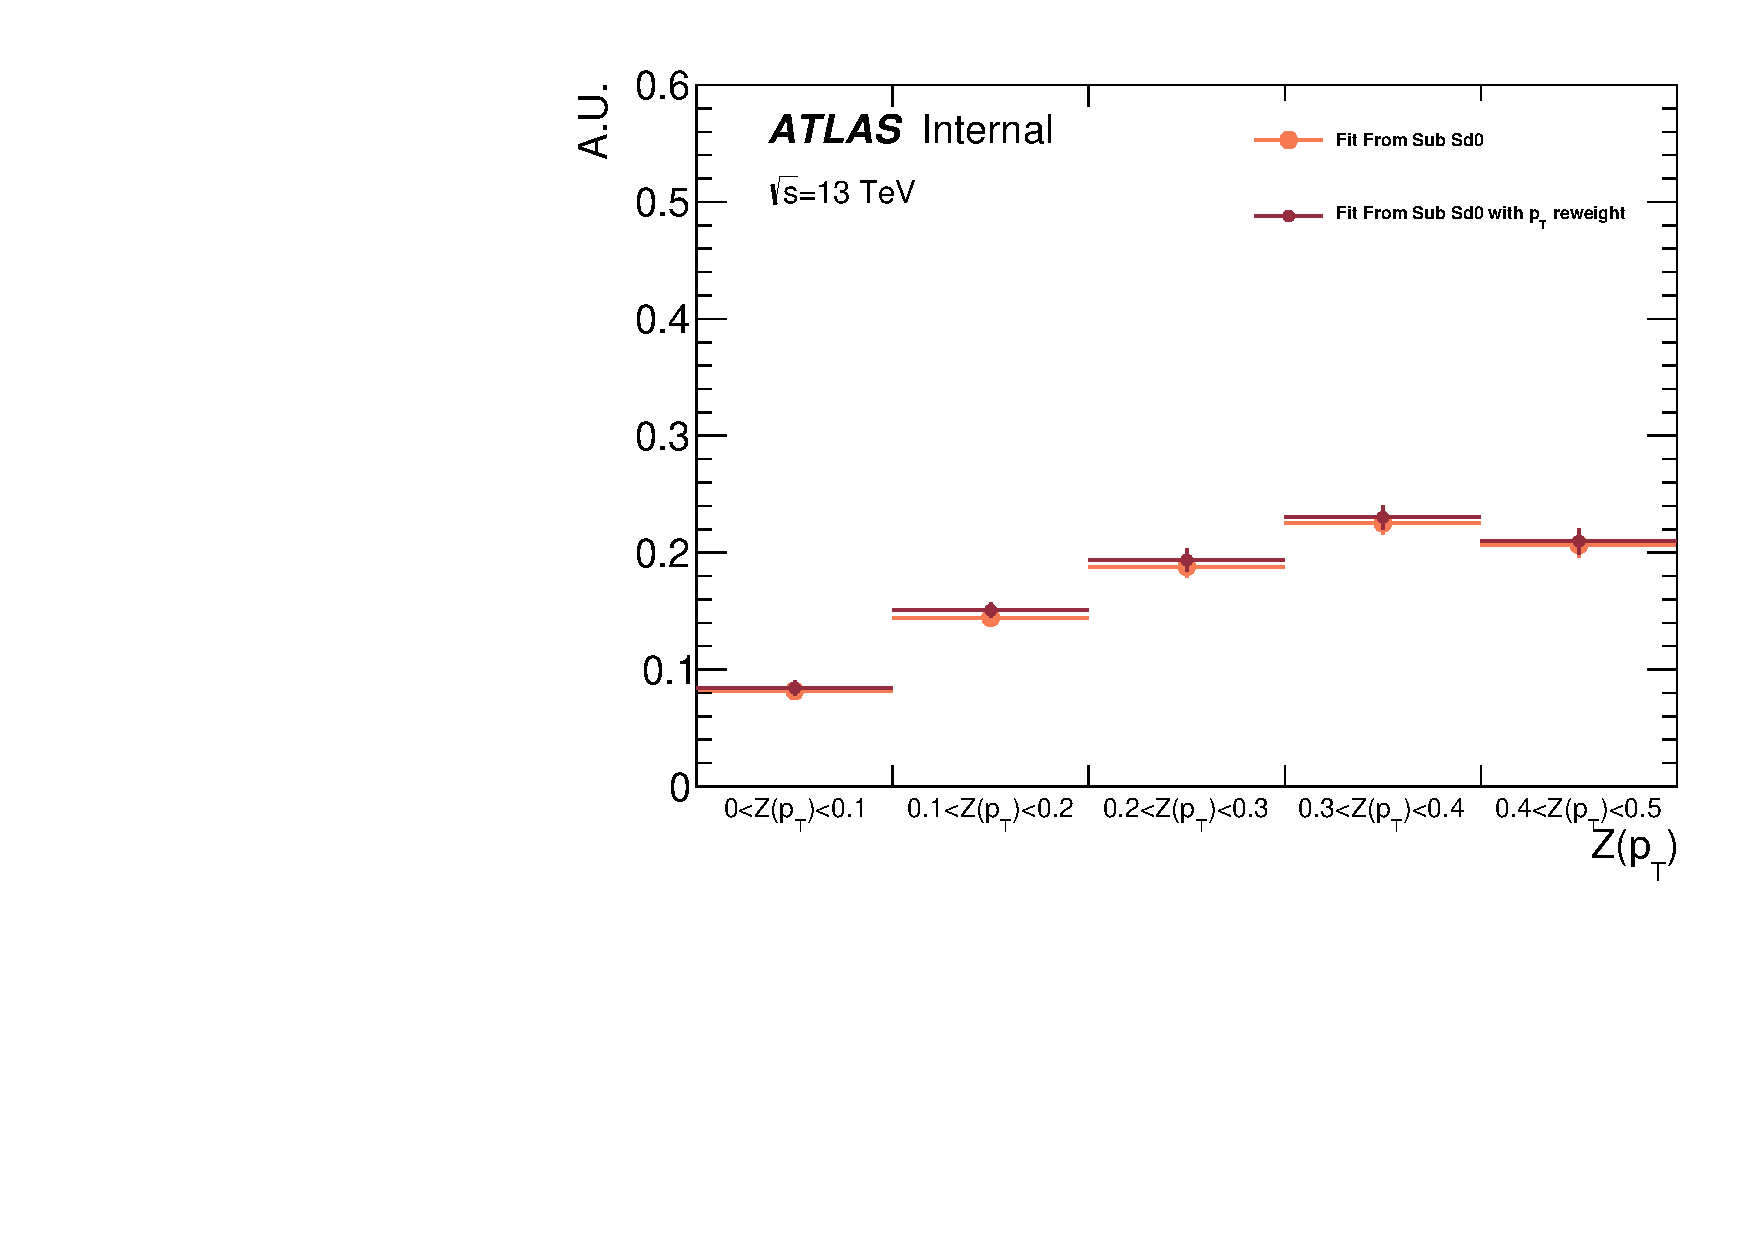
\includegraphics[width=0.45\textwidth]{figures/gbb/Sub_Sd0_Fits/Canv_ZpT_noreweightCrossCheck.pdf}\\
\caption{Comparison of flavor fractions fitted (1) using \subsdzero and \sdzero (top left), (2) using \subsdzero and \subsubsdzero (top right), (3) using inclusive and $p_T$ parameterized templates (bottom left) and (4) with and without track jet kinematic re-weighting (bottom right) in bins of \zpt}
  \label{fig:ZpT-fitfrac-crosscheck}
\end{figure}


\begin{figure}[htbp]
  \centering
 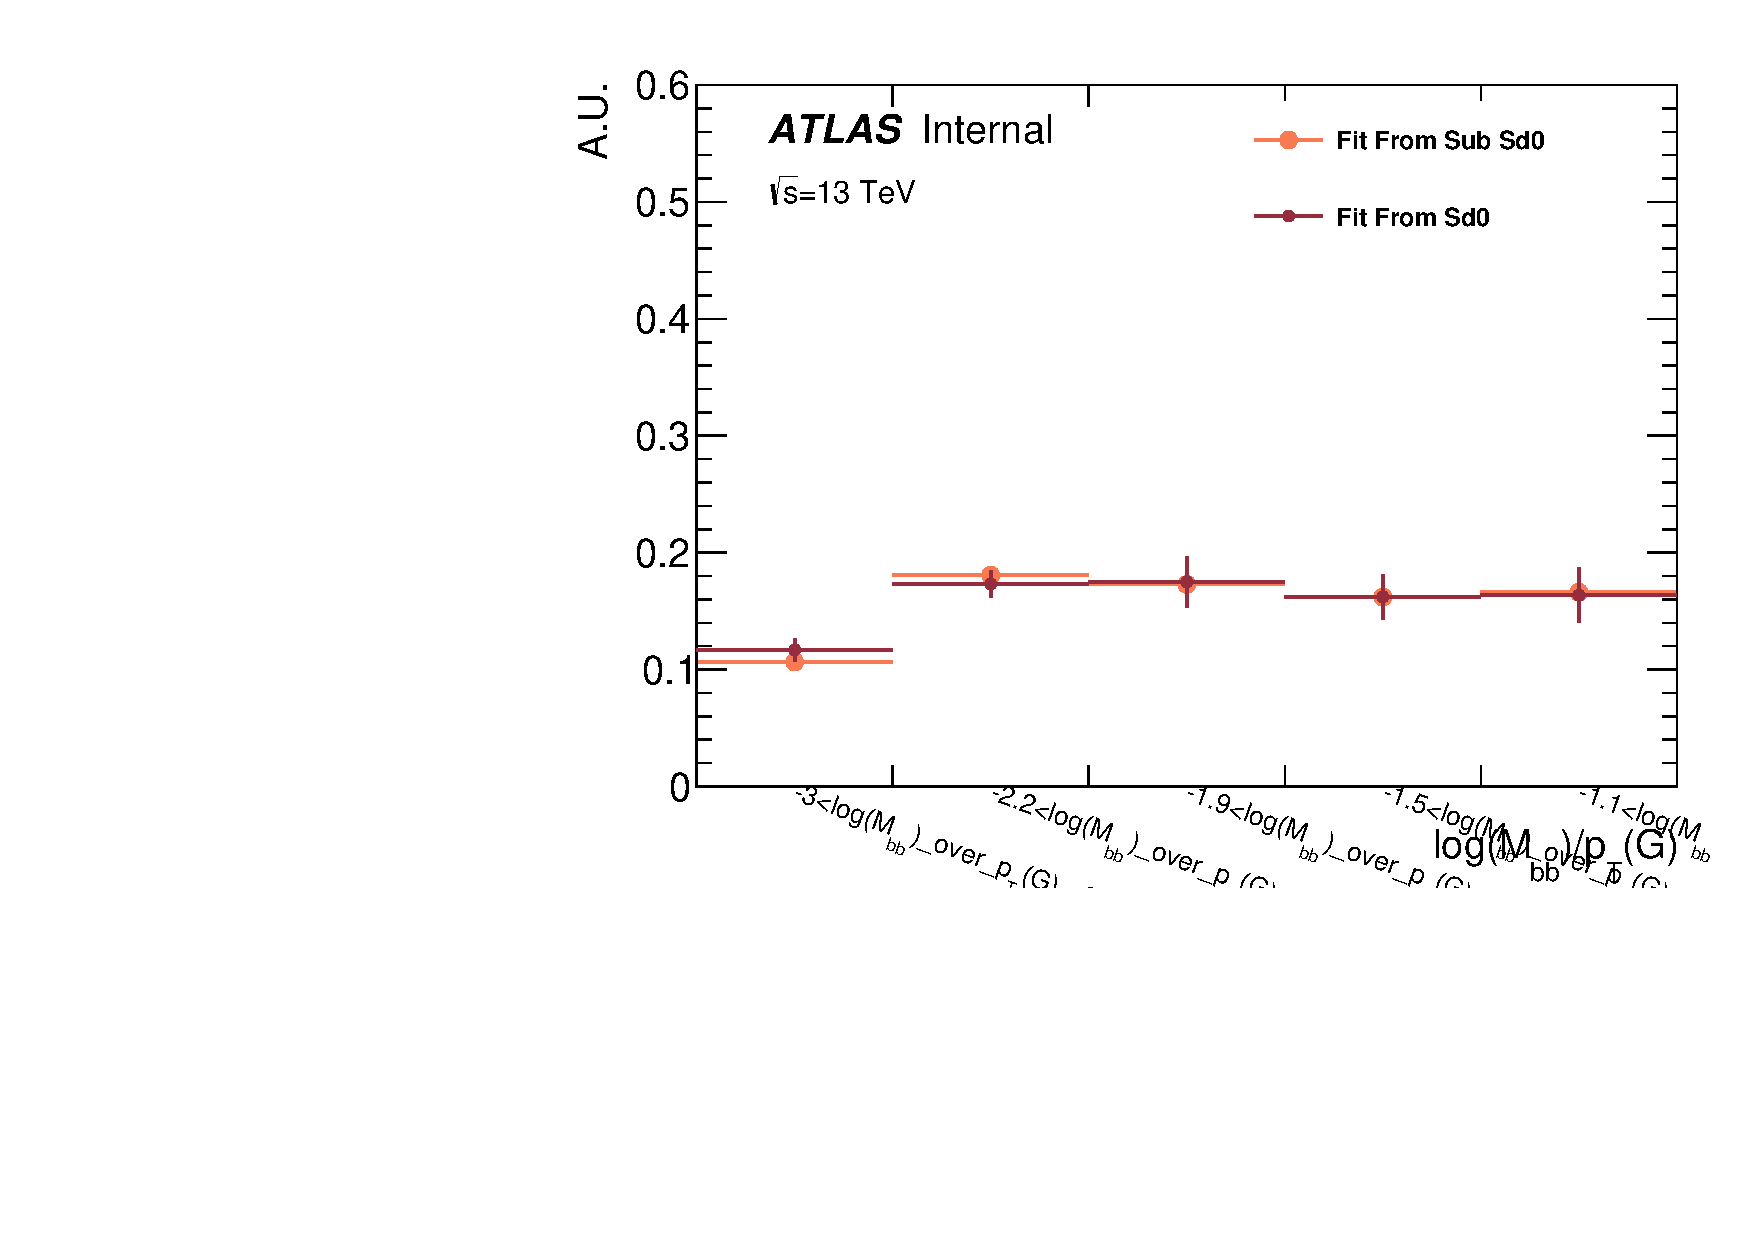
\includegraphics[width=0.45\textwidth]{figures/gbb/Sub_Sd0_Fits/Canv_fracmasspt_leadCrossCheck.pdf}
 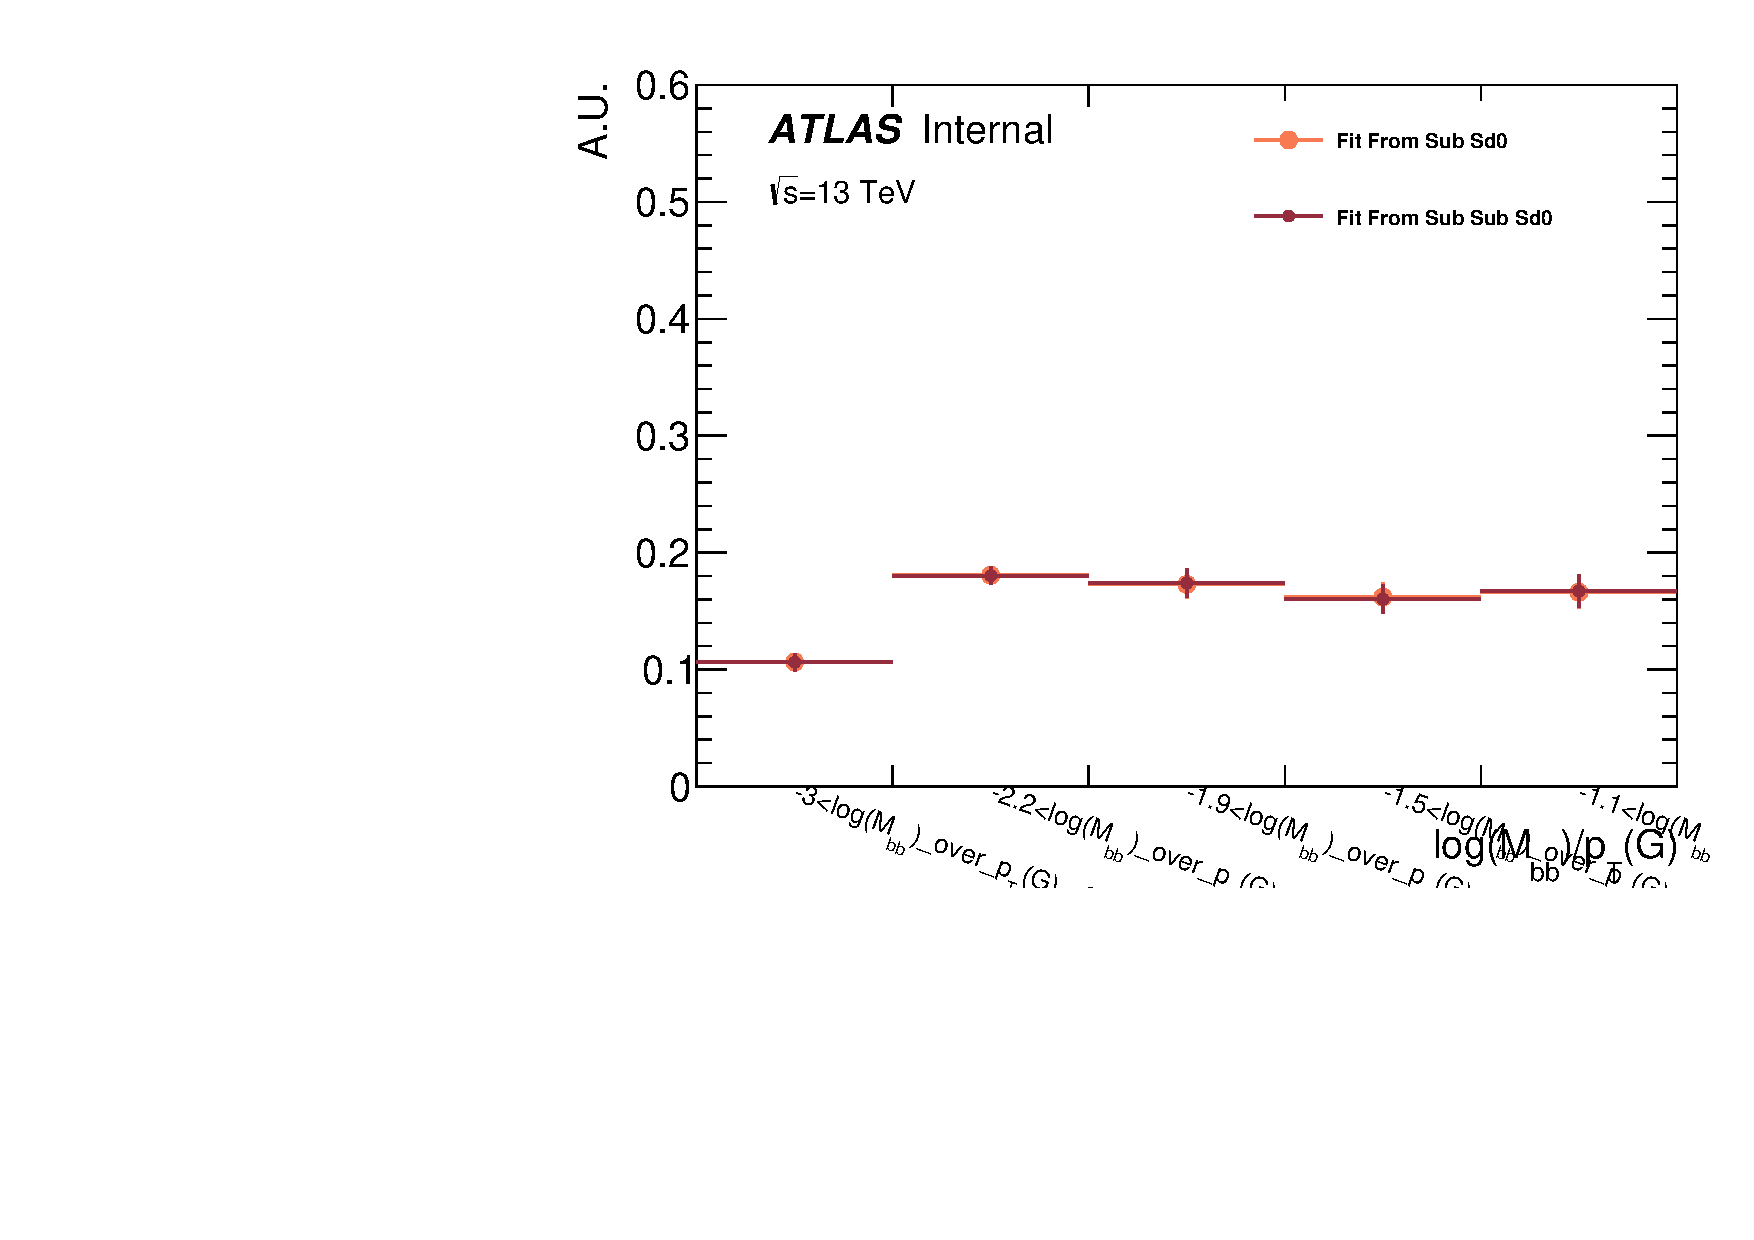
\includegraphics[width=0.45\textwidth]{figures/gbb/Sub_Sd0_Fits/Canv_fracmasspt_subsubCrossCheck.pdf}\\
 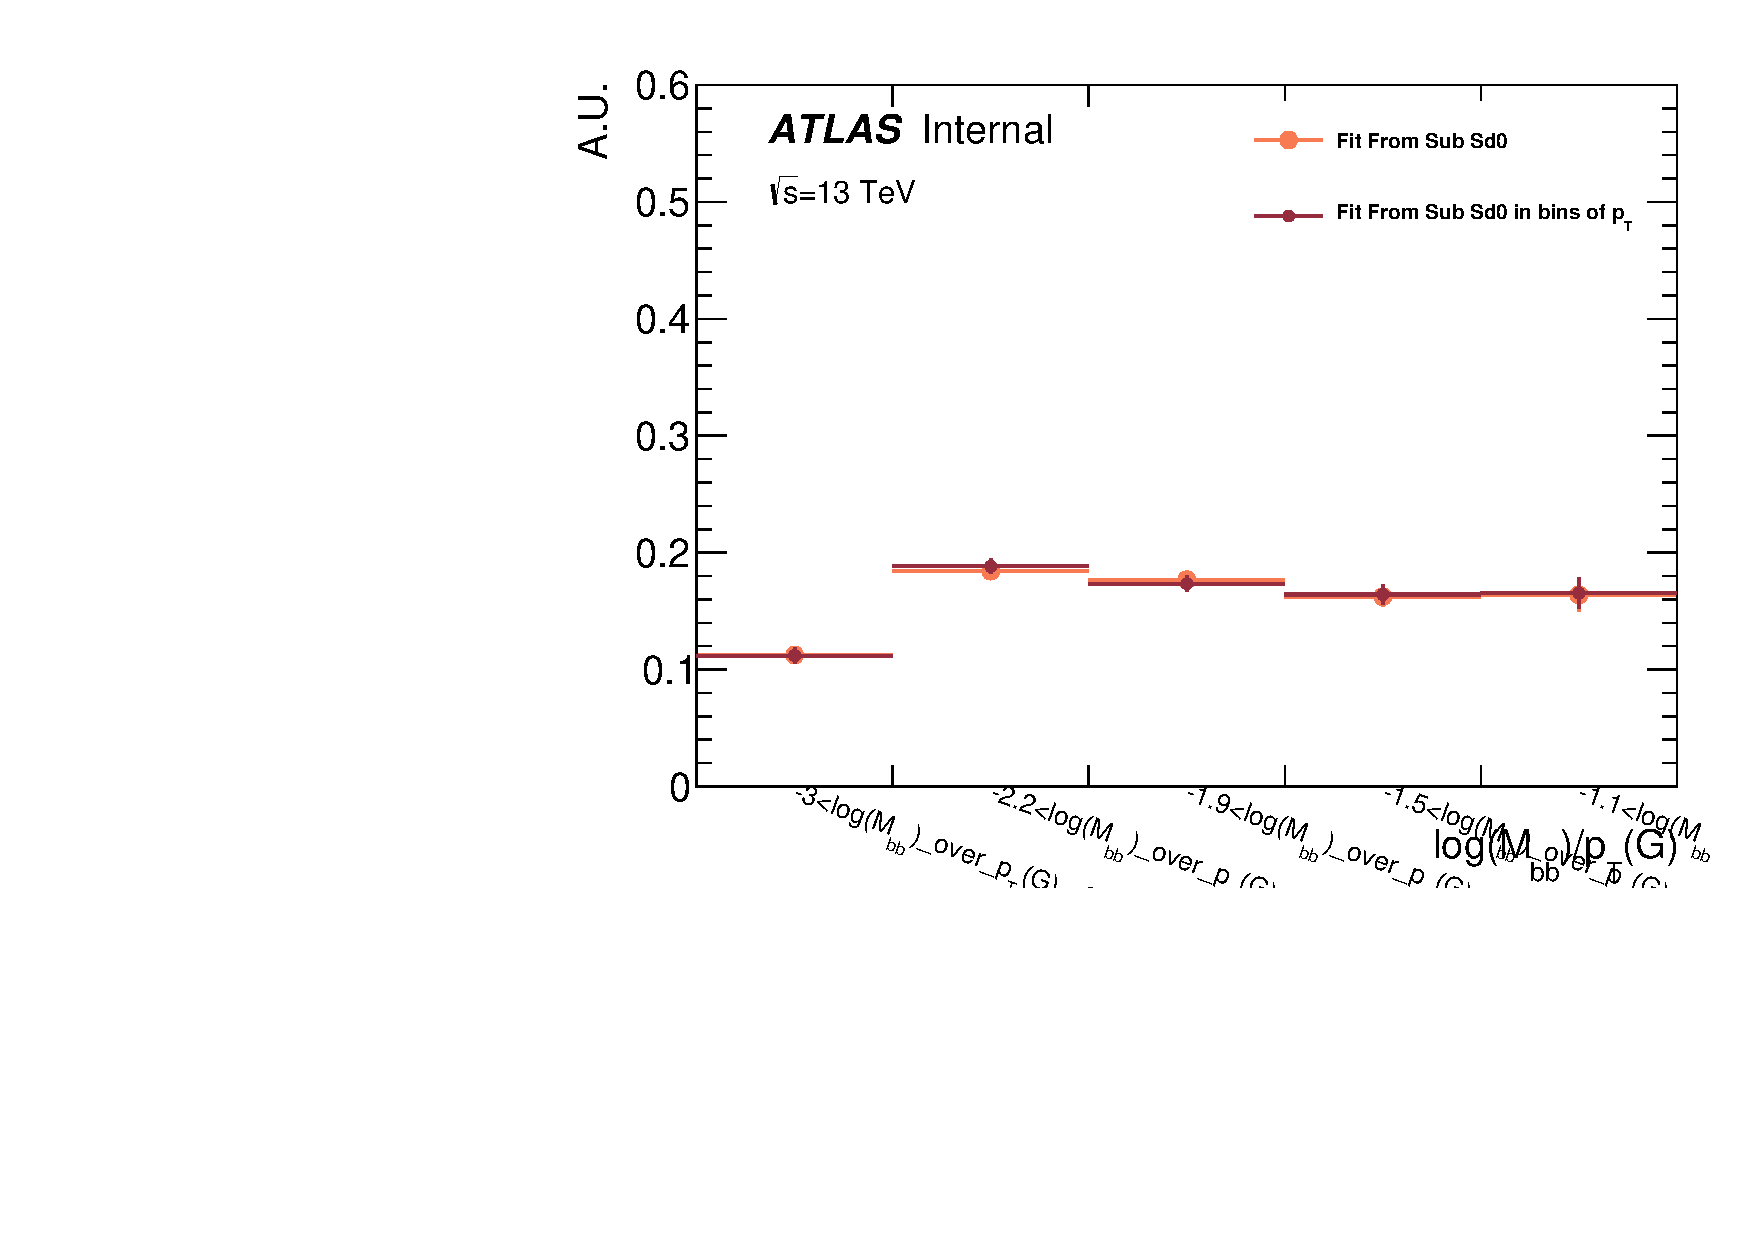
\includegraphics[width=0.45\textwidth]{figures/gbb/Sub_Sd0_Fits/Canv_fracmasspt_ptbinCrossCheck.pdf}
 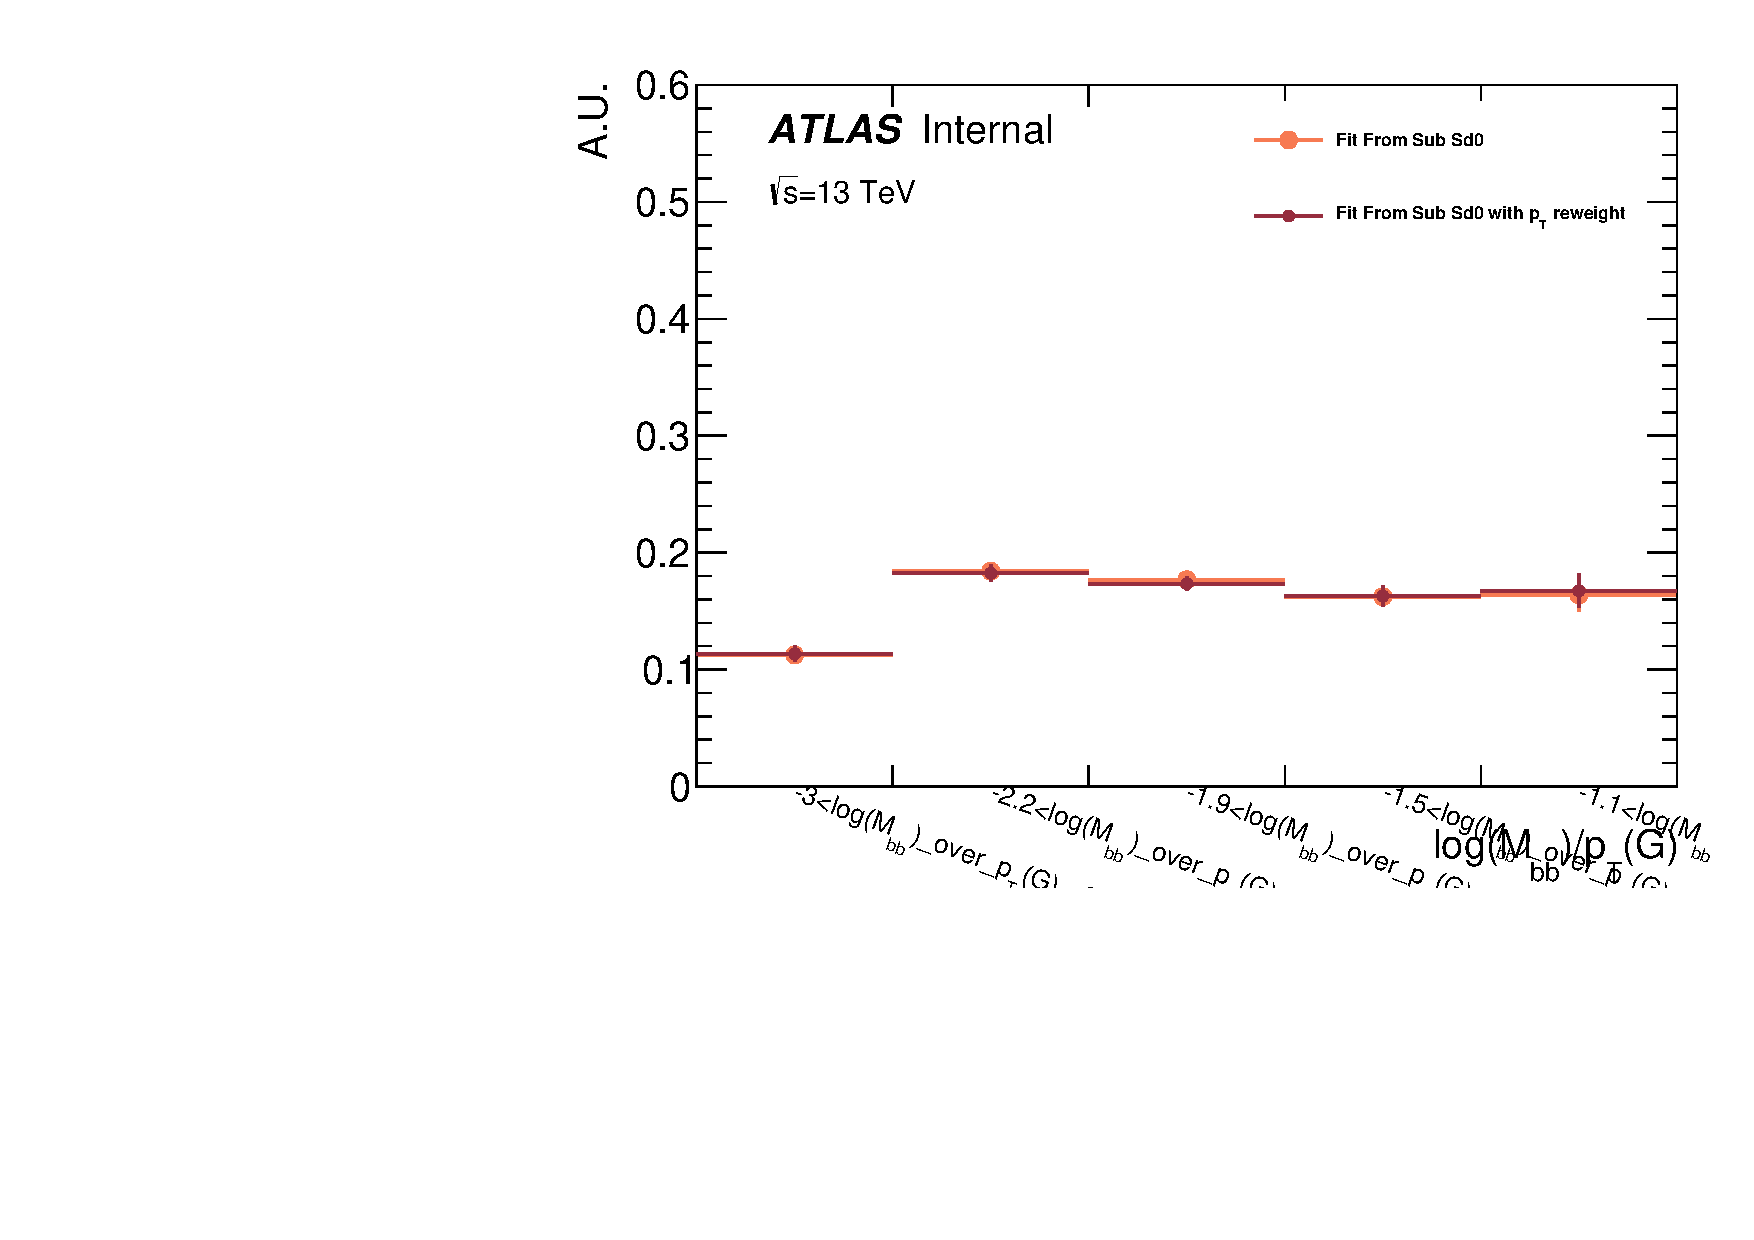
\includegraphics[width=0.45\textwidth]{figures/gbb/Sub_Sd0_Fits/Canv_fracmasspt_noreweightCrossCheck.pdf}\\
\caption{Comparison of flavor fractions fitted (1) using \subsdzero and \sdzero (top left), (2) using \subsdzero and \subsubsdzero (top right), (3) using inclusive and $p_T$ parameterized templates (bottom left) and (4) with and without track jet kinematic re-weighting (bottom right) in bins of \mpt}
  \label{fig:fracmasspt-fitfrac-crosscheck}
\end{figure}

\begin{figure}[htbp]
  \centering
 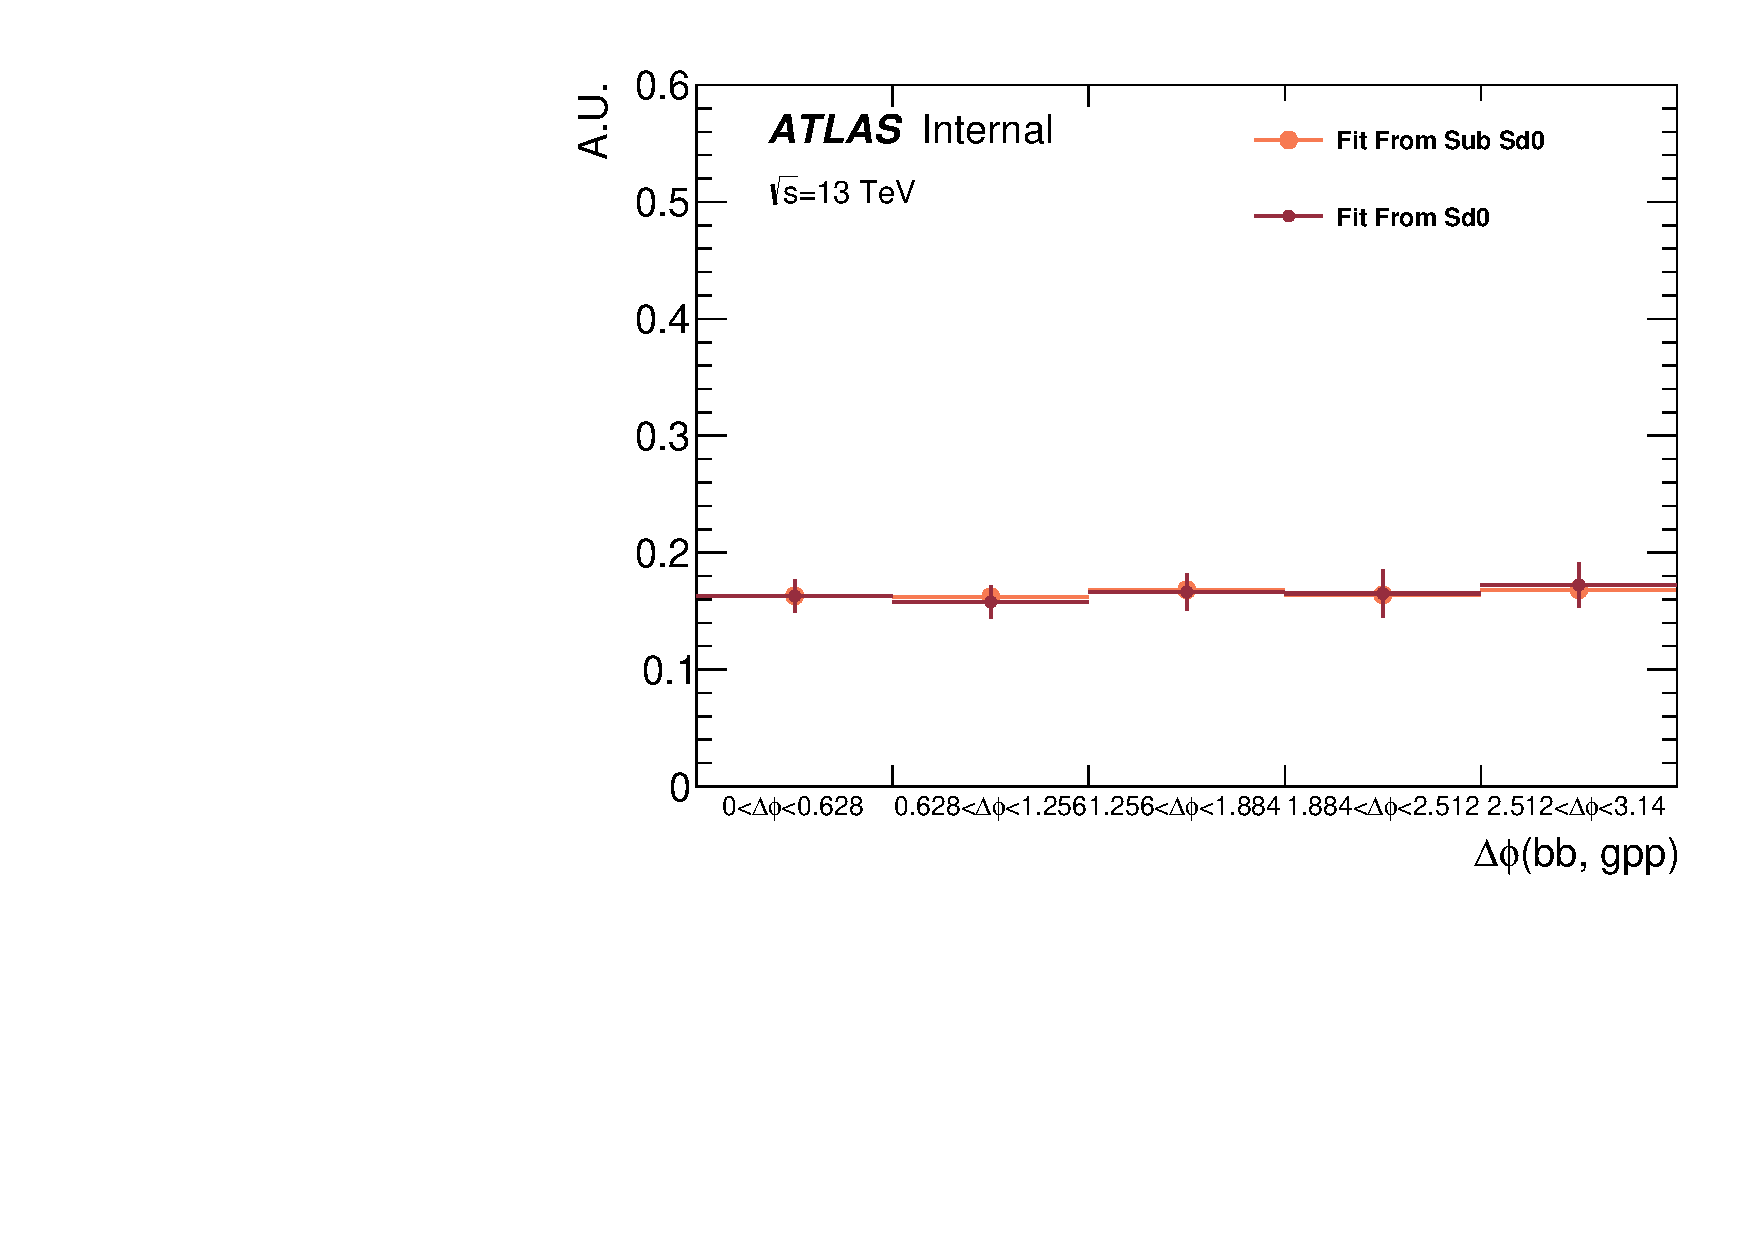
\includegraphics[width=0.45\textwidth]{figures/gbb/Sub_Sd0_Fits/Canv_dphi_leadCrossCheck.pdf}
 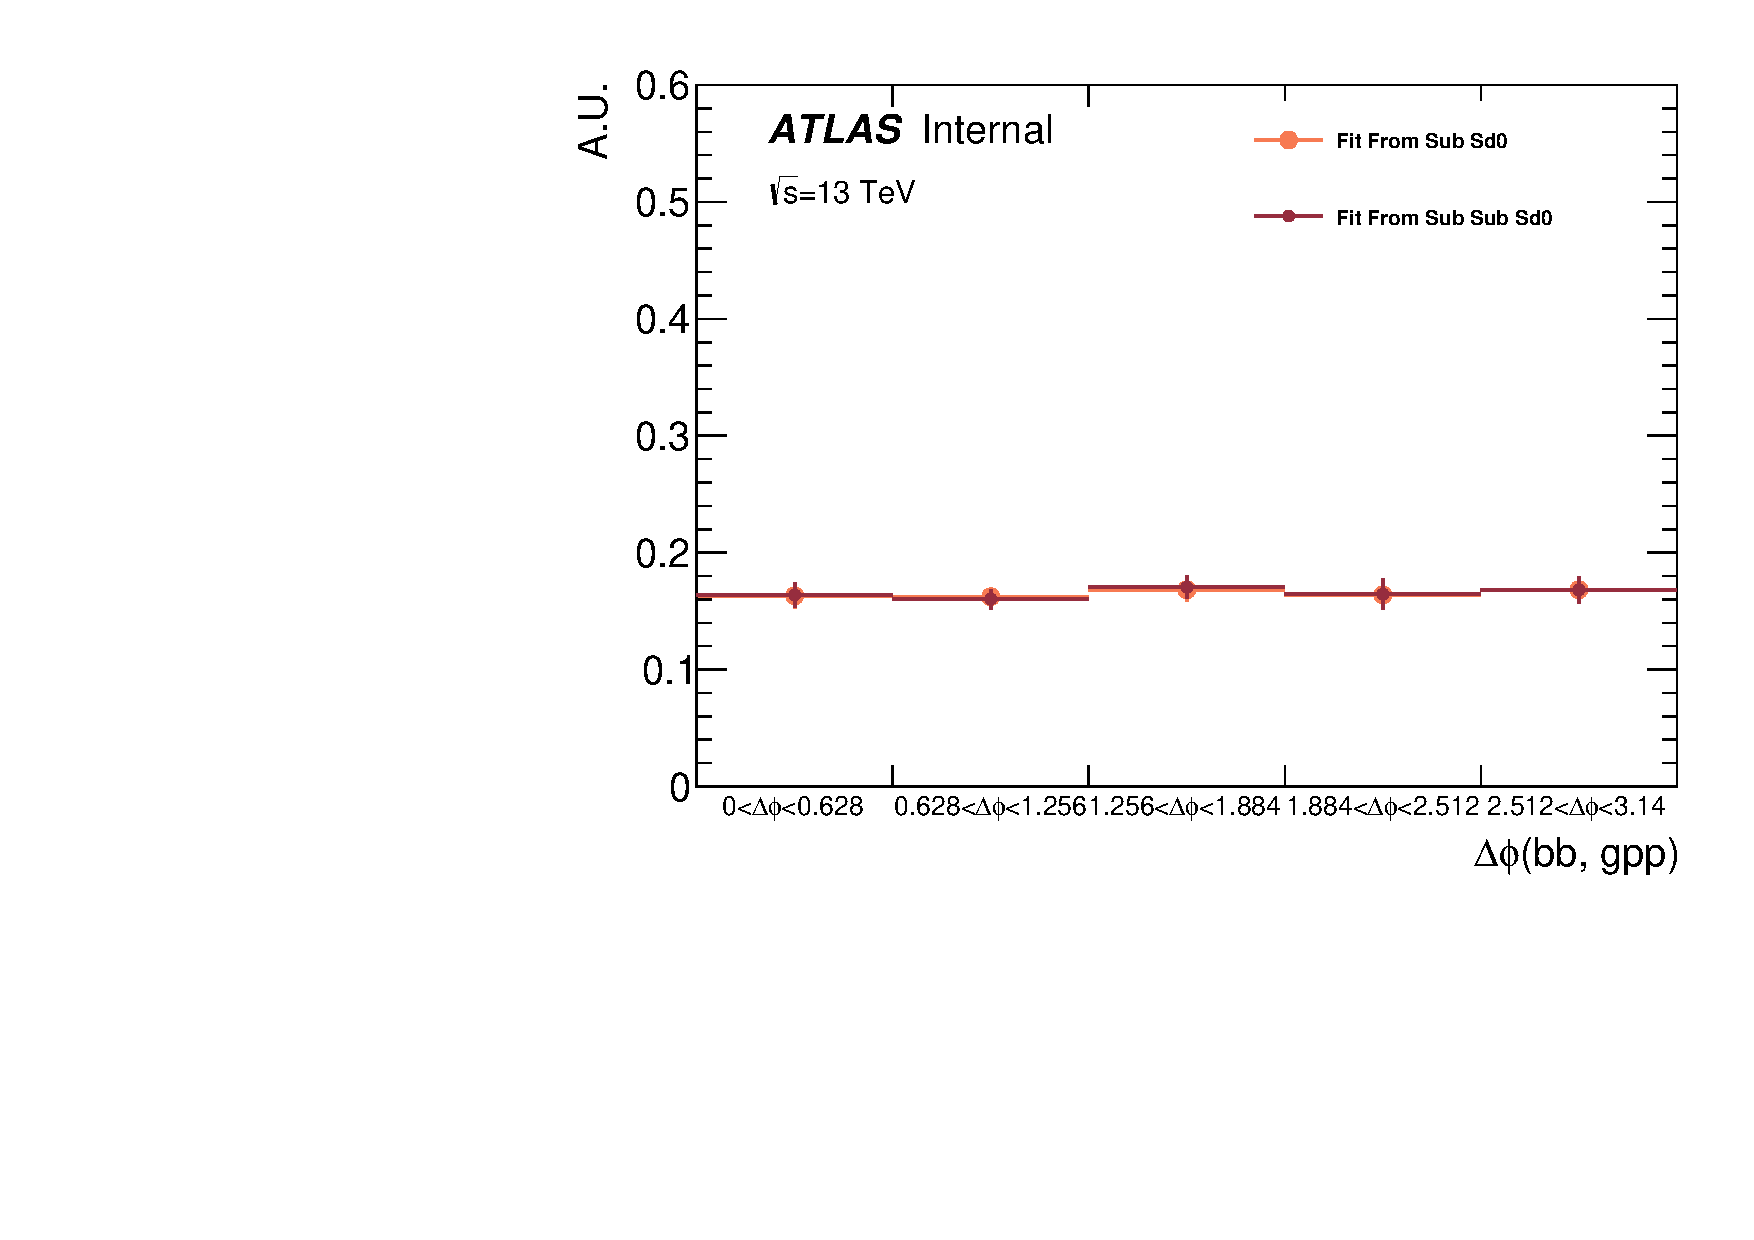
\includegraphics[width=0.45\textwidth]{figures/gbb/Sub_Sd0_Fits/Canv_dphi_subsubCrossCheck.pdf}\\
 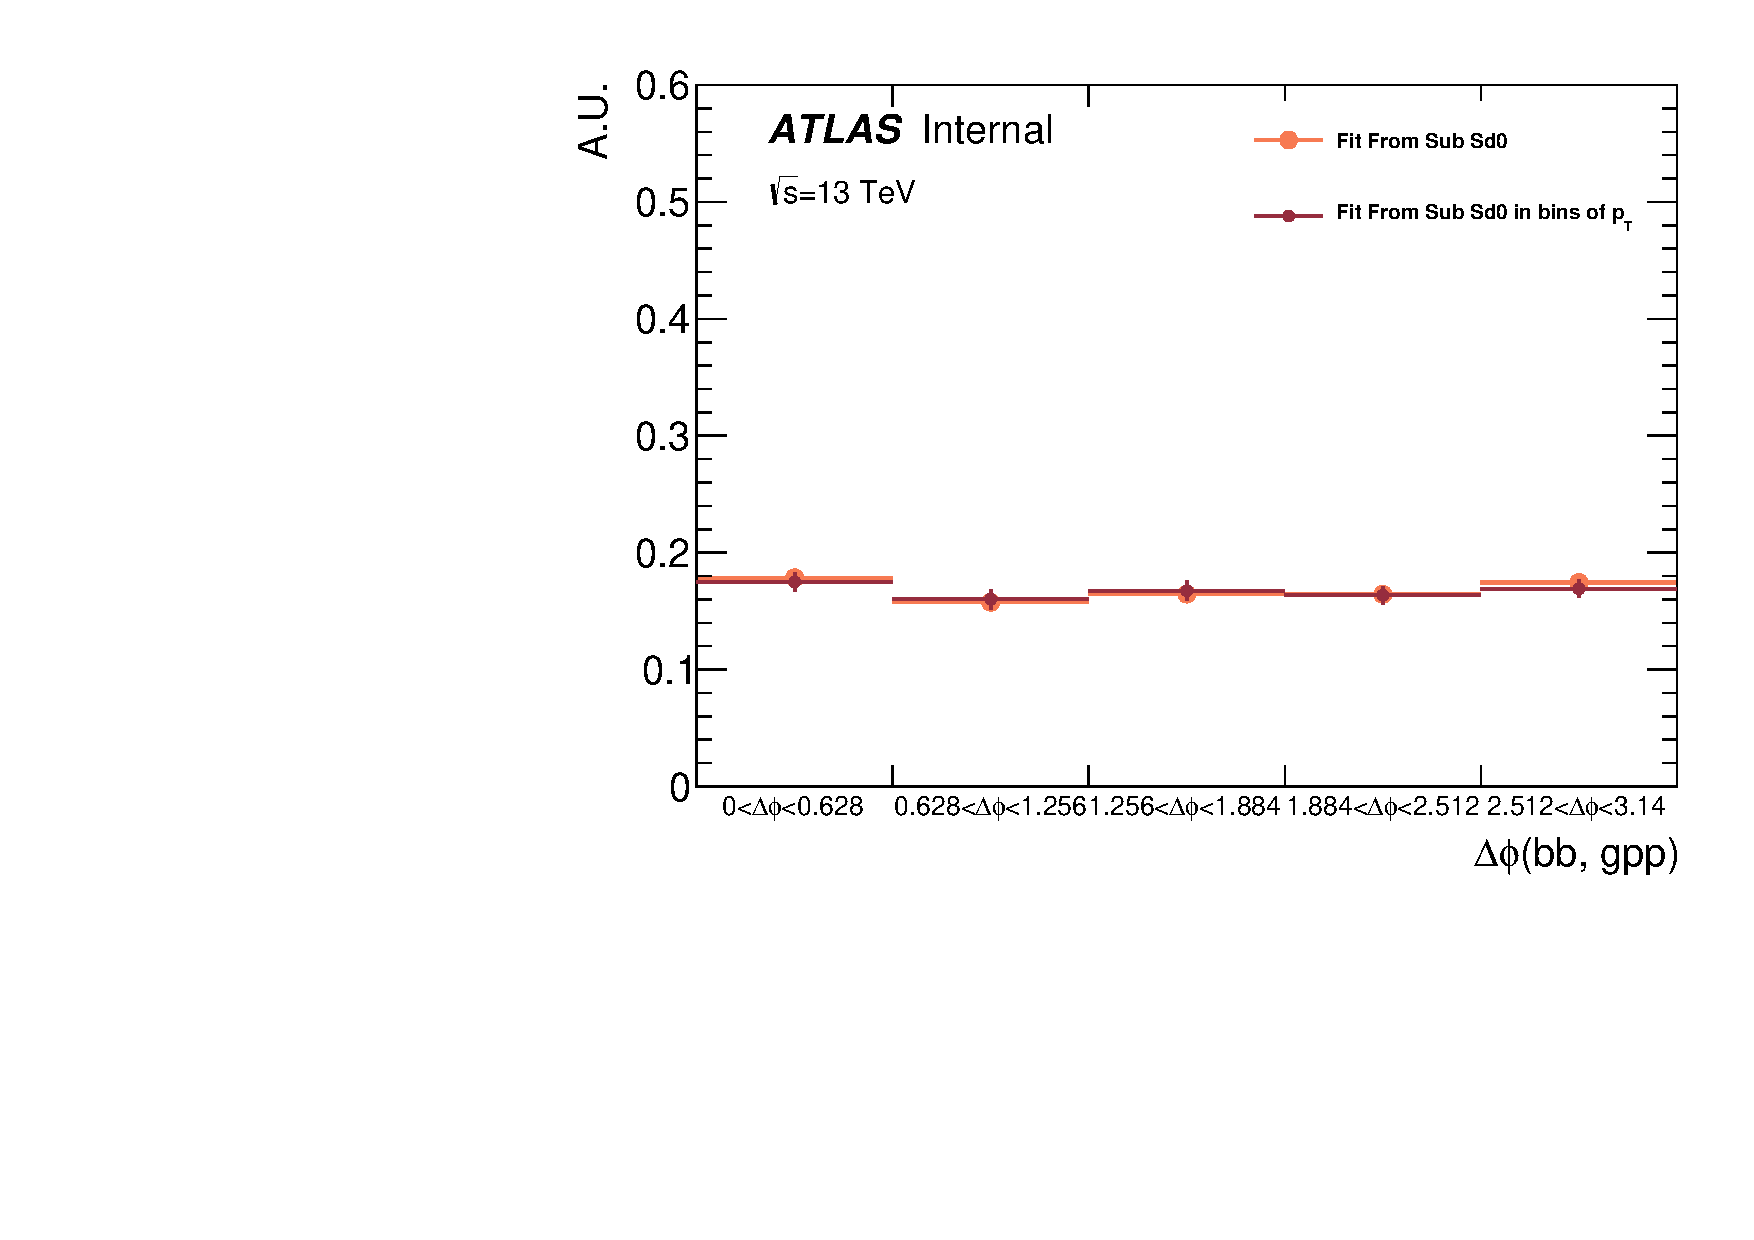
\includegraphics[width=0.45\textwidth]{figures/gbb/Sub_Sd0_Fits/Canv_dphi_ptbinCrossCheck.pdf}
 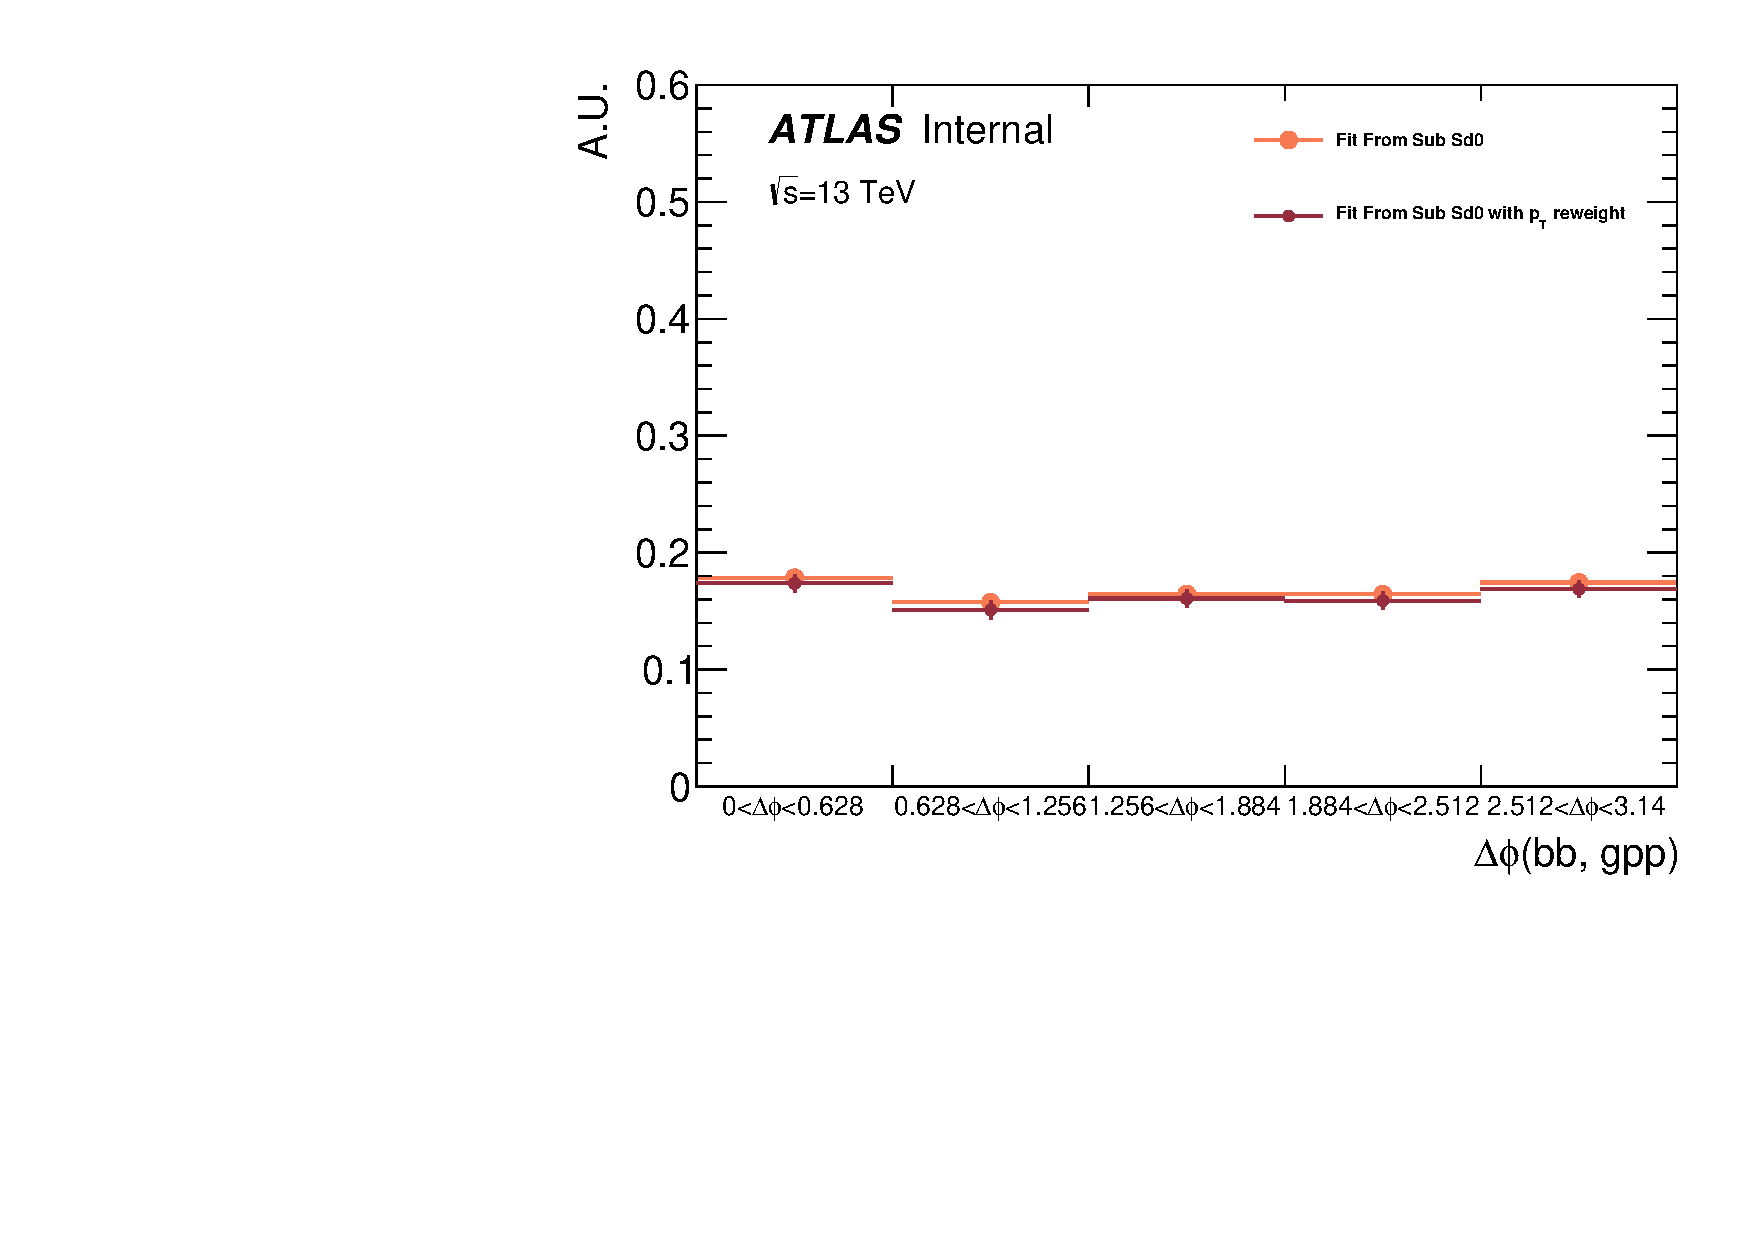
\includegraphics[width=0.45\textwidth]{figures/gbb/Sub_Sd0_Fits/Canv_dphi_noreweightCrossCheck.pdf}\\
\caption{Comparison of flavor fractions fitted (1) using \subsdzero and \sdzero (top left), (2) using \subsdzero and \subsubsdzero (top right), (3) using inclusive and $p_T$ parameterized templates (bottom left) and (4) with and without track jet kinematic re-weighting (bottom right) in bins of \dphi}
  \label{fig:dphi-fitfrac-crosscheck}
\end{figure}


\clearpage

